%!TEX TS-program = xelatex
%!TEX encoding = UTF-8 Unicode
\documentclass[10pt, parindent=0]{article} % use larger type; default would be 10pt

%----------------------------------------------------------------------------------------
%   PACKAGES
%----------------------------------------------------------------------------------------
\usepackage[parfill]{parskip}
\usepackage{amsmath,amsfonts,amsthm} % Math packages
\usepackage{mathtools}
\usepackage{lipsum} % Used for inserting dummy 'Lorem ipsum' text into the template
\usepackage{datetime}
\usepackage{xfrac}
\usepackage{changepage} % for adjusting the width
\usepackage{gensymb}
\usepackage{subcaption}
\usepackage{sectsty}
\usepackage{xcolor}
\usepackage{verbatim}
\usepackage{titlesec}
\usepackage{color}
\usepackage{fixltx2e} %helps the [H] problem! 10/2/2015
\usepackage{float} % Not have your figures fly around  - use [H]
\usepackage{booktabs} % for much better looking tables
\usepackage{array} % for better arrays (e.g matrices) in maths
\usepackage{paralist} % very flexible & customisable lists (eg. enumerate/itemize, etc.)
\usepackage{verbatim} % adds environment for commenting out blocks of text & for better verbatim
\usepackage{subfig} % make it possible to include more than one captioned figure/table in a single float
\usepackage[export]{adjustbox}
\usepackage{pdfpages} % For pdf inputs
\usepackage{import} % for subfolder inputs
\usepackage{metalogo} % for the fucking logo
\usepackage{listings}
\usepackage{mdwlist} % for tight lists
\usepackage{csquotes} % provide the \enquote command for quick quotes
%\usepackage{import} % for subfolder inputs
\usepackage{letltxmacro} % better roots
\usepackage{xspace} % for correct spacing
\usepackage{multicol} % for the multicol environment
%\usepackage{hyperref}
\usepackage{sidecap} % for sided captions
\usepackage{wrapfig}

% enable system font access
\usepackage{fontspec}

% nomenclature
\usepackage{nomencl}
\makenomenclature %change position
%----------------------------------------------------------------------------------------
%   FONT CONFIGURATIONS
%----------------------------------------------------------------------------------------

\setmainfont{Palatino Linotype}
\newfontfamily{\maintext}{Palatino Linotype}
\newfontfamily{\stressed}{Helvetica}
%\newfontfamily\secfont{Arial}
%\newfontfamily{\exotic}{Arial}
%\newfontfamily{\math}{Arial}
\setsansfont{Arial}

%----------------------------------------------------------------------------------------
%   DOCUMENT CONFIGURATIONS
%----------------------------------------------------------------------------------------
\definecolor{MediumBlue}{rgb}{0 ,0 ,205}
\definecolor{Blue}{rgb}{0 ,0 ,255}
\definecolor{RoyalBlue}{rgb}{65,105,225}
\definecolor{mygreen}{rgb}{0,0.6,0}
\definecolor{mygray}{rgb}{0.5,0.5,0.5}
\definecolor{mymauve}{rgb}{0.58,0,0.82}

%\titleformat*{\section}{\bfseries \color{MediumBlue}}
%\titleformat*{\subsection}{\bfseries \color{Blue}}
%\titleformat*{\subsubsection}{\bfseries \color{RoyalBlue}}
\newcommand{\en}[1] {\textenglish{#1}}

\titleformat{\paragraph}
{\normalfont\normalsize\bfseries}{\theparagraph}{1em}{}
\titlespacing*{\paragraph}
{0pt}{3.25ex plus 1ex minus .2ex}{1.5ex plus .2ex}

% New Root configuration - http://en.wikibooks.org/wiki/LaTeX/Mathematics#Roots
\LetLtxMacro{\oldsqrt}{\sqrt} % makes all sqrts closed
\renewcommand{\sqrt}[1][\ ]{%
  \def\DHLindex{#1}\mathpalette\DHLhksqrt}
\def\DHLhksqrt#1#2{%
  \setbox0=\hbox{$#1\oldsqrt[\DHLindex]{#2\,}$}\dimen0=\ht0
  \advance\dimen0-0.2\ht0
  \setbox2=\hbox{\vrule height\ht0 depth -\dimen0}%
  {\box0\lower0.71pt\box2}}

\newcommand{\norm}[1]{\lVert#1\rVert}
\newcommand{\abs}[1]{\lvert#1\rvert}

%% Tensors  command
\newcommand*{\rttensor}[1]{\underline{\underline{#1}}}

%----------------------------------------------------------------------------------------
%   GEOMETRY - GRAPHICS 
%----------------------------------------------------------------------------------------
\usepackage[a4paper, width = 150mm, top = 25mm, bottom = 25mm, bindingoffset =
5mm]{geometry} % to change the page dimensions
\usepackage{graphicx} % support the \includegraphics command and options

\graphicspath{ 
{./Drawings/CameraUploads/}
{./Drawings/MoreFigures/}
{./Drawings/Figures/}
{./Drawings/MatlabFigures/}
}

%----------------------------------------------------------------------------------------
%   LISTINGS RELATED
%----------------------------------------------------------------------------------------

\lstset{ %
  backgroundcolor=\color{white},   % choose the background color; you must add \usepackage{color} or \usepackage{xcolor}
  basicstyle=\footnotesize,        % the size of the fonts that are used for the code
  breakatwhitespace=false,         % sets if automatic breaks should only happen at whitespace
  breaklines=true,                 % sets automatic line breaking
  captionpos=t,                    % sets the caption-position to bottom
  commentstyle=\color{mygreen},    % comment style
  deletekeywords={...},            % if you want to delete keywords from the given language
  escapeinside={\%*}{*)},          % if you want to add LaTeX within your code
  extendedchars=true,              % lets you use non-ASCII characters; for 8-bits encodings only, does not work with UTF-8
  frame=none,                    % adds a frame around the code
  keepspaces=true,                 % keeps spaces in text, useful for keeping indentation of code (possibly needs columns=flexible)
  keywordstyle=\color{blue},       % keyword style
  language=Matlab,                 % the language of the code
  morekeywords={*,...},            % if you want to add more keywords to the set
  numbers=none,                    % where to put the line-numbers; possible values are (none, left, right)
  numbersep=5pt,                   % how far the line-numbers are from the code
  numberstyle=\tiny\color{mygray}, % the style that is used for the line-numbers
  rulecolor=\color{black},         % if not set, the frame-color may be changed on line-breaks within not-black text (e.g. comments (green here))
  showspaces=false,                % show spaces everywhere adding particular underscores; it overrides 'showstringspaces'
  showstringspaces=false,          % underline spaces within strings only
  showtabs=false,                  % show tabs within strings adding particular underscores
  stepnumber=2,                    % the step between two line-numbers. If it's 1, each line will be numbered
  stringstyle=\color{mymauve},     % string literal style
  tabsize=2,                       % sets default tabsize to 2 spaces
  title=\lstname                   % show the filename of files included with \lstinputlisting; also try caption instead of title
}

\newcommand{\includecode}[2][c]{\lstinputlisting[caption=#2, escapechar=, style=custom#1]{#2}}

% numbering only some equations in an align* environment
\newcommand\numberthis{\addtocounter{equation}{1}\tag{\theequation}}
  % then use \eqref{eqn_label}


%----------------------------------------------------------------------------------------
%   HEADER & FOOTERS
%----------------------------------------------------------------------------------------
\usepackage{fancyhdr} % This should be set AFTER setting up the page geometry
\pagestyle{fancy} % options: empty , plain , fancy
\renewcommand{\headrulewidth}{0.4pt} % customise the layout...
\lhead{\textcolor{gray}{Flight Mechanics}\\
\textcolor{gray}{Aerodynamic and Control analysis of J35 Draken}}\chead{}\rhead{\textcolor{gray}{Nikolaos Koukis}}
\lfoot{}\cfoot{\thepage}\rfoot{}

%----------------------------------------------------------------------------------------
%   SECTION APPEARANCE
%----------------------------------------------------------------------------------------
% (This matches ConTeXt defaults)
\numberwithin{equation}{section} % Number equations within sections (i.e. 1.1, 1.2, 2.1, 2.2 instead of 1, 2, 3, 4)
\numberwithin{figure}{section} % Number figures within sections (i.e. 1.1, 1.2, 2.1, 2.2 instead of 1, 2, 3, 4)
\numberwithin{table}{section} % Number tables within sections (i.e. 1.1, 1.2, 2.1, 2.2 instead of 1, 2, 3, 4)

%----------------------------------------------------------------------------------------
%   TOC APPEARANCE
%----------------------------------------------------------------------------------------
\usepackage[nottoc,notlof,notlot]{tocbibind} % Put the bibliography in the ToC

%----------------------------------------------------------------------------------------
%   DOCUMENT PART
%----------------------------------------------------------------------------------------
\begin{document}
%----------------------------------------------------------------------------------------
%   TITLE SECTION
%----------------------------------------------------------------------------------------
\newcommand{\horrule}[1]{\rule{\linewidth}{#1}} % Create horizontal rule command with 1 argument of height

\begin{titlepage}

\begin{center}
\begin{figure}[htpb]
    \begin{center}
        
\includegraphics[width = 0.2\textwidth]{kth_rgb.jpg} % Just THIS!!!
    \end{center}
\end{figure}

\normalfont \normalsize 
\textsc{Royal Institute of Technology} \\  % Your university, school and/or department name(s)
\textsc{School of Engineering Sciences} \\ [25pt] % Your university, school and/or department name(s)
\horrule{0.5pt} \\[0.4cm] % Thin top horizontal rule
\huge Flight Mechanics \vspace{5mm}\\ Project Work Part \\ % The assignment title
\horrule{2pt} \\[0.5cm] % Thick bottom horizontal rule
\vspace*{10mm}

\begin{figure}[H]
    \centering
    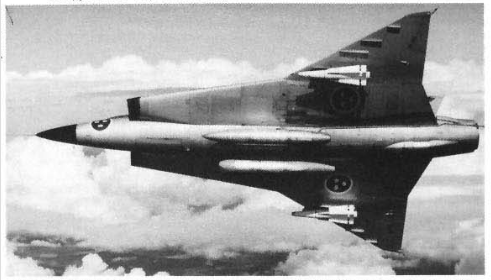
\includegraphics[width=\textwidth]{S35F}
\end{figure}

\LARGE 
Nikolaos Koukis

\vfill
\normalsize \normalfont
Personnummer: 930727T073\\
Date delivered: 2015/02/03\\
Group: D
\end{center}
\end{titlepage}

\newpage
\tableofcontents
\listoffigures
%\lstlistoflistings
\newpage

%%%%%%%%%%%%%%%%%%%%%%%%%%%%%%%%%%%%%%%
%       ABSTRACT-NOMENCLATURE         %
%%%%%%%%%%%%%%%%%%%%%%%%%%%%%%%%%%%%%%%
\section{Abstract}
This is the report for the performance analysis project in the \textit{Flight Mechanics} course
offered by the School of Engineering Sciences at KTH. The report was written using the \textit{Vim} Editor
and the \XeLaTeX typesetting system. For the coding part the \textit{Matlab} technical computing language was used.


\printnomenclature[1cm] % print the nomenclature
 
%%%%%%%%%%%%%%%%%%%%%%%%%%%%%%%%%%%%%%%
%           INTRODUCTION              %
%%%%%%%%%%%%%%%%%%%%%%%%%%%%%%%%%%%%%%%
%\section{Introduction}

\subsection{General Characteristics}
As the jet era started, Sweden foresaw the need for a jet fighter that could intercept bombers at high 
altitude and also successfully engage fighters. Although other interceptors such as the 
US Air Force's F-104 Starfighter were being conceived during the same period, 
Saab's "Draken" would have to undertake a combat role unique to Sweden. 
Other demanding requirements were the capability to operate from reinforced public roads 
used as part of wartime airbases, and for refuelling/rearming to be 
carried out in no more than ten minutes, by conscripts with minimal training. 
\textbf{In September 1949, the Swedish Defence Material Administration issued a request for a fighter/interceptor aircraft, and work began at Saab the same year}

\textit{Regarding the aerodynamic design of the J35 Draken the two major options were swept wings and delta wings.}
The question was quickly resolved by the initial studies which had called for the
exploration of a swept wing configuration. In short order it  was determined tha
in consideration of all other parameteres placed upon the design, 
the swept wing's aerodynamic drag at high Mach numbers was too high, 
and its configuration requirements dictated that the fuselage have insufficient 
volume for equipment, fuel and armament.
The Delta wing on the other hand showed great promise following initial tunnel 
tests. The pure delta soon was ruled out, however, as it suffered from center 
of gravity and center of pressure anomalies that were difficult to alleviate. 
A derivative, however, often referred to as \textit{the double delta}, proved much more flexible. 
In general the double delta was found to offer the attributes of:
\begin{itemize*}
    \item reduced frontal area while permitting optimal wing area
    \item More favorable wing sweep angles on the center wing section
    \item Center of gravity and center of pressure being closer to each other
    \item More favorable area distribution
    \item Low supersonic drag
    \item Favorable low speed drag
    \item Strong and stiff fail safe structure
    \item Being able to place the air intakese farther forward
\end{itemize*}
The double-delta configuration was first tested on the SAAB 210 which first flew
on 21 January 1952.

\begin{figure}[H]
  \centering
  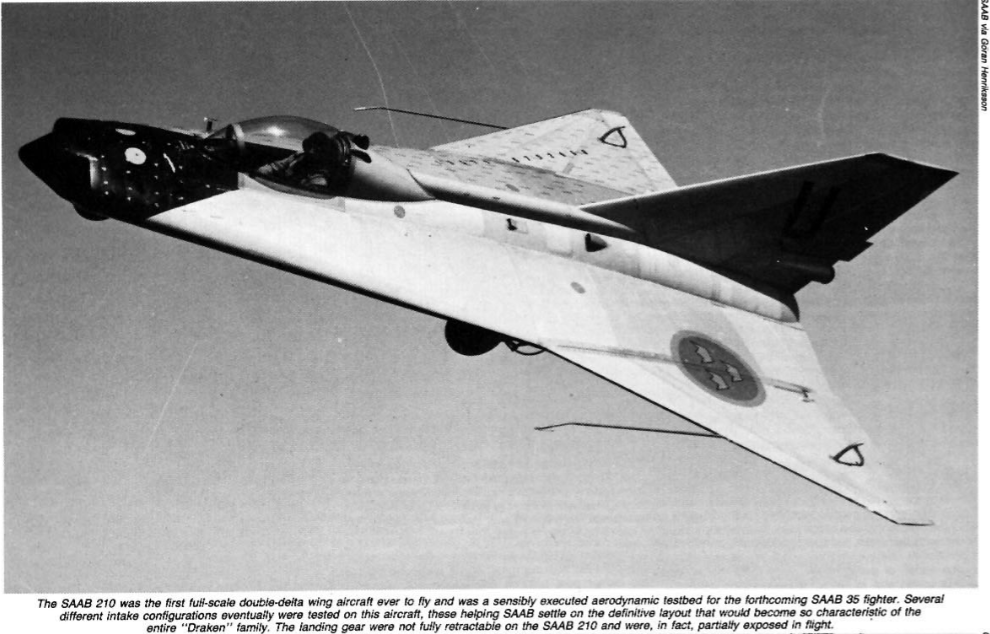
\includegraphics[width=1.2\textwidth]{SAAB210}
  \caption{SAAB 210}
\end{figure}
\begin{figure}[H]
  \centering
  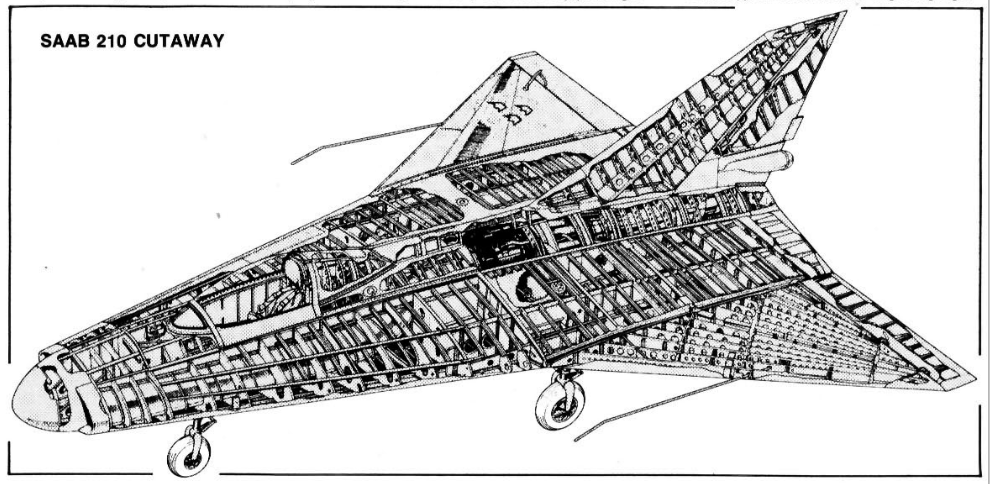
\includegraphics[width=1.3\textwidth]{Cutaway}
  \caption{Cutaway design of SAAB 210}
\end{figure}

\subsection{Basic Versions}

Below are the major versions of J35 Draken which were manufactured from 1955
to 1974 by Saab.
\subsubsection{J35A}

    \begin{itemize*}
        \item First flew on 1958
        \item Total Production: 90
        \item Delivered from 1959 to 1961
    \end{itemize*}

\begin{figure}[H]
  \centering
  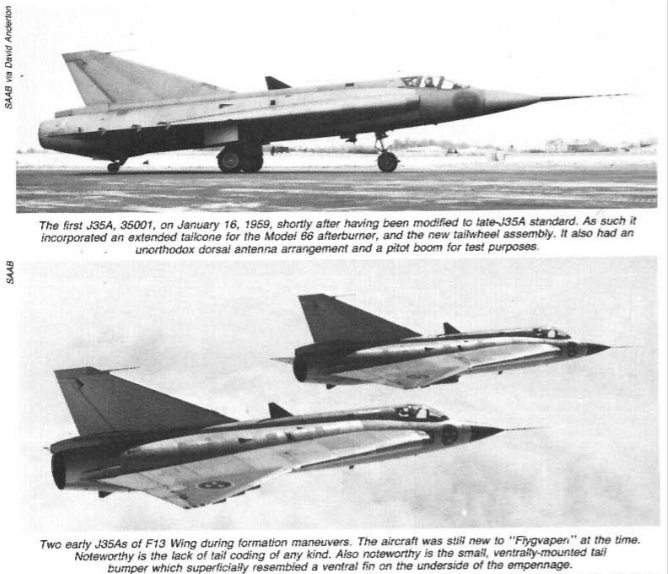
\includegraphics[width=1.0\textwidth]{J35A}
  \caption{J35A}
\end{figure}
\subsubsection{J35B}
\begin{itemize*}
        \item First flew on 1959
        \item Total Production: 73
        \item Delivered from 1962 to 1963
        \item First truly operating interceptor version of J35 Draken
    \end{itemize*}

\begin{figure}[H]
    \centering
    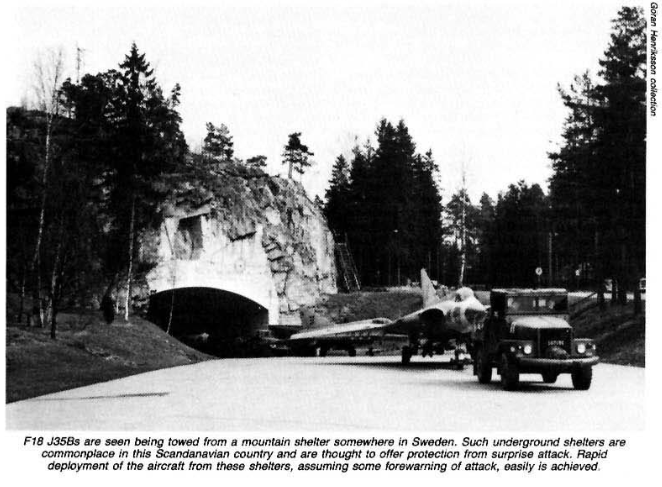
\includegraphics[width=1.0\textwidth]{S35b_sheltered}
    \caption{J35B carried out of sheltered area}
\end{figure}

\begin{figure}[H]
    \centering
    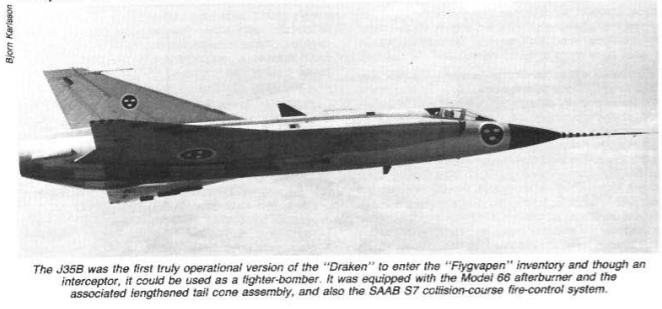
\includegraphics[width=1.0\textwidth]{S35B}
    \caption{J35B}
\end{figure}

\subsubsection{Sk35C}
    \begin{itemize*}
        \item First flew on 1959
        \item Total Production: -
        \item Essentially 25 J35A with short tail sections rebuilt 
            into a twin-seated trainer version
        \item To provide space for a second cockpit some equipment was relocated and the size of the forward
            fuel tank was reduced.
        \item Lacking the guns and radar of single-seater, the Sk35C nevertheless could be 
            used for armament training with Sidewinder missiles and other external stores.
    \end{itemize*}

\begin{figure}[H]
  \centering
  \hspace*{-2cm} 
  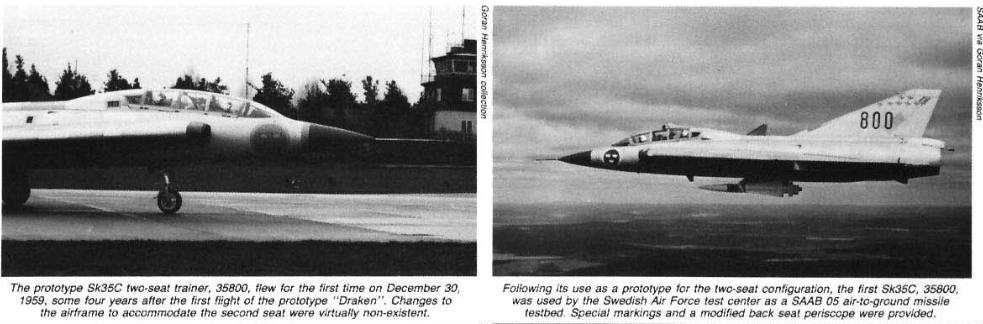
\includegraphics[width=1.2\textwidth]{Sk35C}
  \caption{Sk35C}
\end{figure}

\subsubsection{J35D}
    \begin{itemize*}
        \item First flew on 1960
        \item Total Production: 120
        \item Delivered from 1963 to 1964
        \item Fastest Draken version, capable of accelerating until out of fuel.
        \item Represented a marked improvement over earlier versions both in terms of performance and combat capabillities.
            The former was obtained by replacing the RM5B engine with RM5C (Avon-300 series) thus increasing the max thrust forom 6.850 kgp to 7.750 kgp
            when using the afterburner.
    \end{itemize*}

\begin{figure}[H]
  \centering
  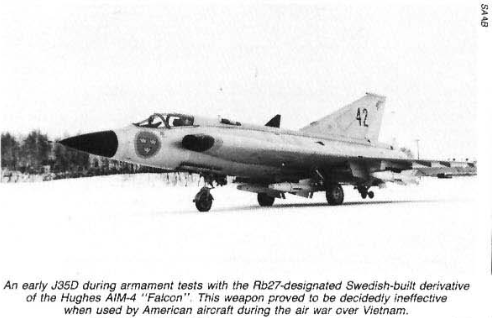
\includegraphics[width=1.0\textwidth]{J35D}
  \caption{J35D}
\end{figure}

\subsubsection{S35E}
    \begin{itemize*}
        \item Total Production: 60
    \end{itemize*}


\begin{figure}[H]
    \centering
    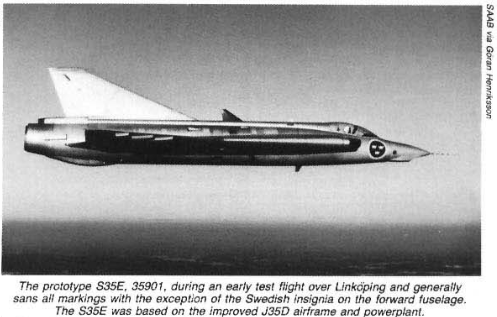
\includegraphics[width=\textwidth]{S35E}
    \caption{J35E}
\end{figure}
\begin{figure}[H]
    \centering
    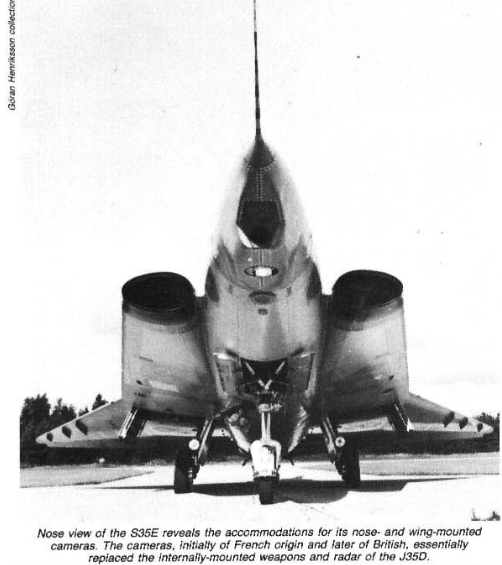
\includegraphics[width=\textwidth]{S35E_b}
    \caption{J35E nose view}
\end{figure}

\subsubsection{S35F}
\begin{figure}[H]
    \centering
    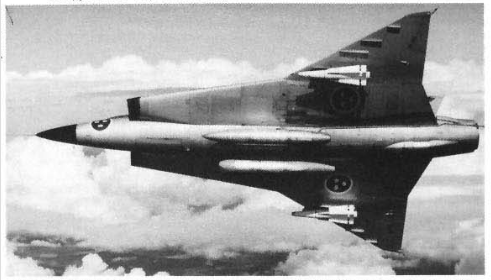
\includegraphics[width=\textwidth]{S35F}
    \caption{J35F}
\end{figure}
\begin{figure}[H]
    \centering
    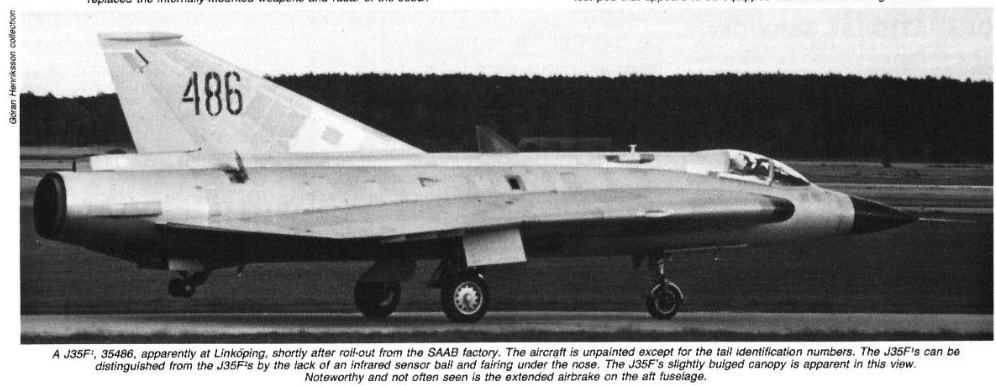
\includegraphics[width=\textwidth]{S35F_b}
    \caption{J35F landing}
\end{figure}

\subsubsection{S35H}
Version of J35 which was supposed to be sold to Switzerland by SAAB. During 1960 it 
was evaluated thoroughly in Switzerland with generally favorable results.
The J35H was not however the only aircraft considered and in the end the Schweizerische
Fliegertruppe concluded that a slightly modified version of Dassault Mirage III was more ideally suited.

\subsubsection{SAAB 35XD}
\begin{itemize*}
    \item Company designation in which X stoood for export and D for Denmark
    \item In 1968 The Danish Goverment ordered 20 single seated 3 two seated trainers 
        23 photo-reconnaissance aircrafts in a follow up order. Finally the Danes revised their offer for 20 single seat 
        20 reconnaisance aircrafts and 11 two-seat trainers.
\end{itemize*}

\subsubsection{SAAB 35XS}
\begin{itemize*}
    \item Export version for Suomi or Finland
    \item Ordered during 1970 by Finland
\end{itemize*}
 %nope.. dont want it
\section{Introduction}

The \textit{SAAB J 35 Draken} was originally conceived as a replacement for the Swedish
Air Force’s venerable \textit{J 29 Tunnan}, an aircraft that was the equivalent of the
F-86 Sabre and MiG-15 in its capabilities, range, performance and load.

Regarding the aerodynamic design of the J35 Draken the two major options
to chose from were swept wings and delta wings \cite{dorr_aerofax_1987}.
The question was quickly resolved by the initial studies which had called
for the exploration of a swept wing configuration. In short order it  was
determined tha in consideration of all other parameteres placed upon the
design, the swept wing's aerodynamic drag at high Mach numbers was too high,
and its configuration requirements dictated that the fuselage have
insufficient volume for equipment, fuel and armament. The pure delta was
also ruled out, however, as it suffered from center of gravity and center of
pressure anomalies that were difficult to alleviate.  A derivative, however,
often referred to as \textit{the double delta}, proved much more flexible.

In general the double delta was found to offer the attributes of:
\begin{itemize*}
    \item Reduced frontal area while permitting optimal wing area
    \item More favorable wing sweep angles on the center wing section
    \item Center of gravity and center of pressure being closer to each other
    \item More favorable area distribution
    \item Low supersonic drag
    \item Favorable low speed drag
    \item Strong and stiff fail safe structure
    \item Being able to place the air intakese farther forward
\end{itemize*}

The plane’s fuselage was a  predictable tube with the engine mounted inside and
the cockpit at the front and a vertical stabilizer attached to the
tail~\cite{riseofDraken}.  The
pointed nose cone contained a radar system and the air intakes for the engine
were on either side of the cockpit at the forward point of the wing root.  The
double-delta began at the air intakes — for roughly two thirds of way toward the
tips, the sweep back measured an incredibly sharp 80 degrees.  This allowed the
plane to achieve design speeds that were in excess of Mach 2.0.  However, with
such a sharp sweep, it was recognized that the plane would be seriously lacking
in maneuverability.  Thus, the last one third of the wings toward the tips
carried a completely different sweep angle, much shallower at 60 degrees.  This
brought excellent maneuverability and enhanced control at low speeds.



%%%%%%%%%%%%%%%%%%%%%%%%%%%%%%%%%%%%%%%
%  PERFORMANCE CHARACTERISTICS        %
%%%%%%%%%%%%%%%%%%%%%%%%%%%%%%%%%%%%%%%
\section{Performance Characteristics of J35 Draken}
%%%%%%%%%%%%%%%%%%%%%%%%%%%%%%%%%%%%%%%
%        STATIC ANALYSIS              %
%%%%%%%%%%%%%%%%%%%%%%%%%%%%%%%%%%%%%%%
\subsection{Static Perfomance}

\subsection{Excess Thrust}

Figure \ref{fig:Tex_Graph} shows the Excess Thrust with regards to the Mach number is presented:

\begin{figure}[H]
    \centering
    \hspace*{-2cm}
    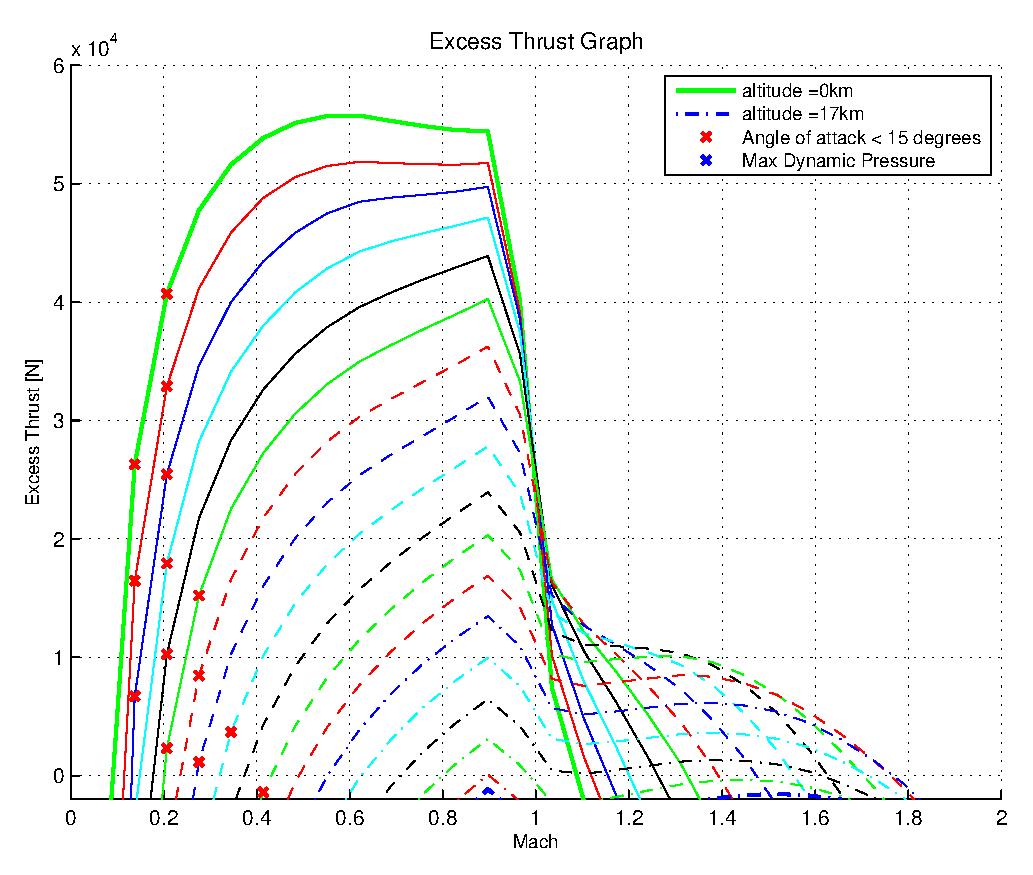
\includegraphics[width=1.2\textwidth]{Tex_Graph}
    \caption{Excess Thrust Graph}
    \label{fig:Tex_Graph}
\end{figure}

Using the graph we can now determine the envelope limits corresponding to the dynamic pressure and the 
maximum angle of attack. These limits are shown in the diagram as red and blue Xs.
We should note however that the dynamic pressure limits are not visible in  \ref{fig:Tex_Graph}, when presenting 
only the part of the diagram above the zero horizontal line, so a supplementary graph (\ref{fig:Tex_Graph2}) is given:

\begin{figure}[H]
    \centering
    \hspace*{-2cm}
    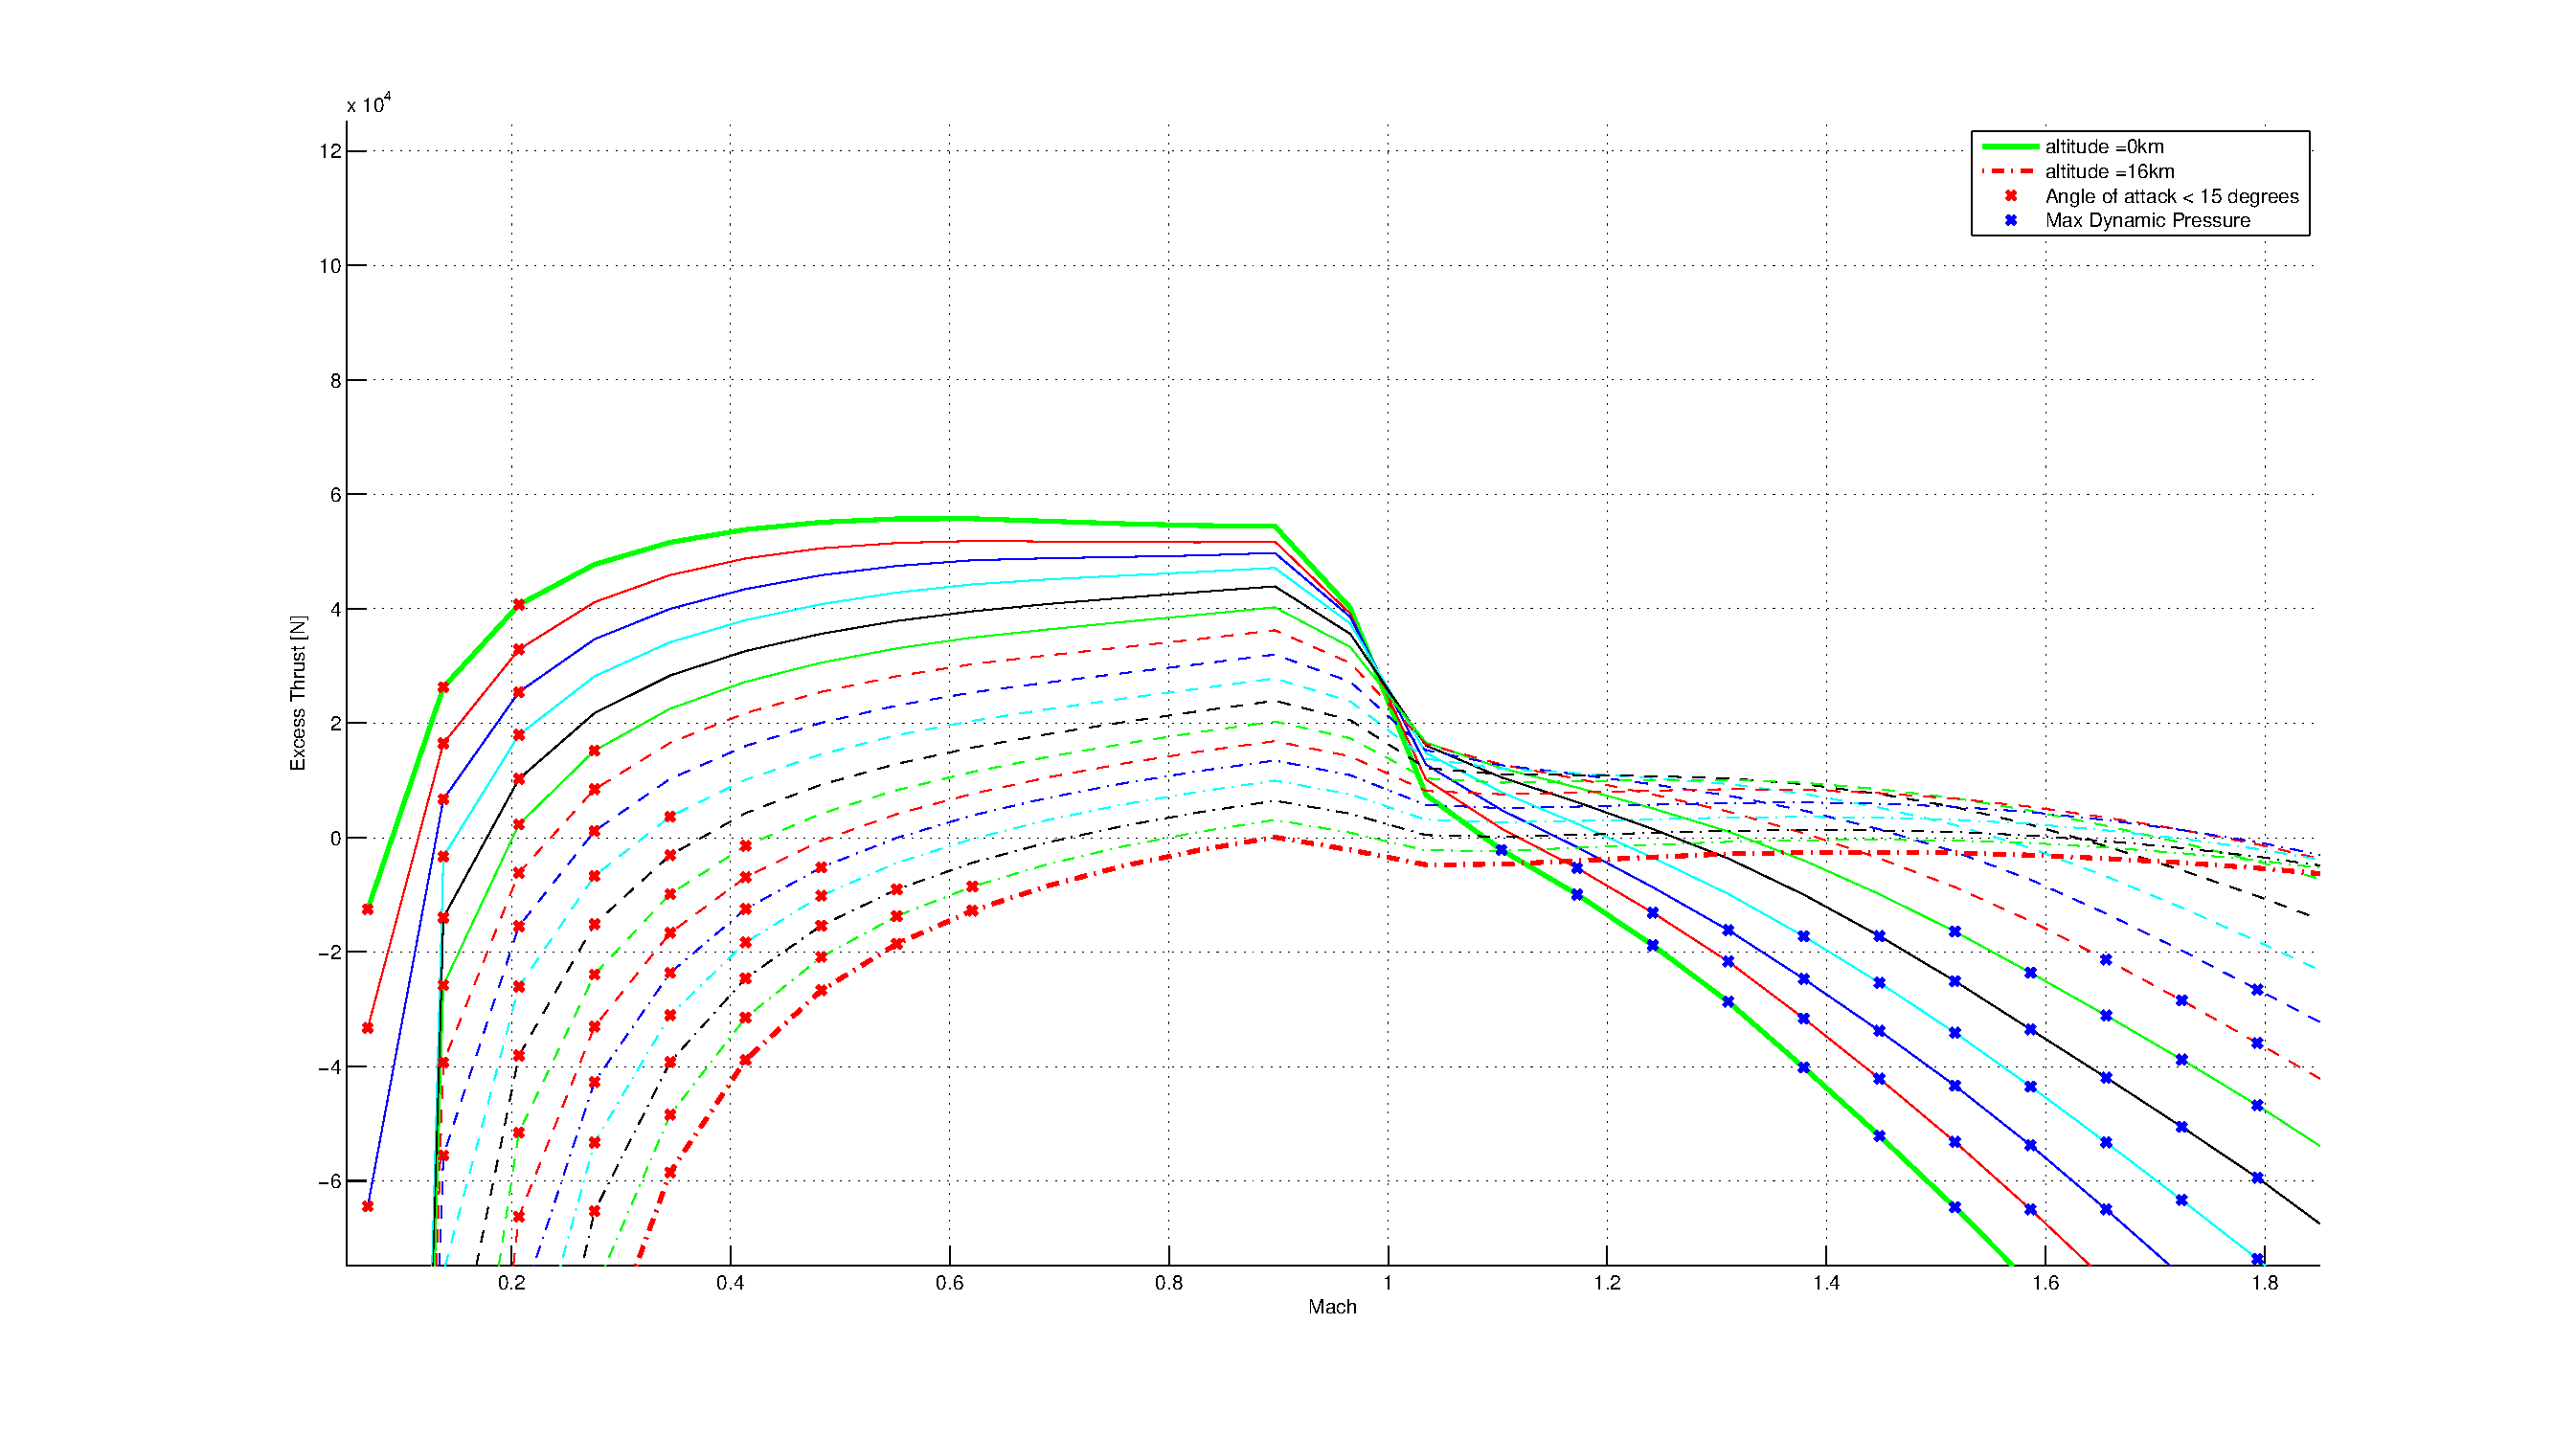
\includegraphics[width=1.2\textwidth]{Tex_Graph2}
    \caption{Excess Thrust Graph - Dynamic pressure limits Visible}
    \label{fig:Tex_Graph2}
\end{figure}

\noindent For the calculation of the Excess Thrust the TexSep function was used. Refer to the TexSep.m module 
for more information on the implementation

\subsection{SEP Graph}

Using the code provided with the report the Specific Excess Power (SEP) Graph
can be plotted:

\begin{figure}[H]
    \centering
    \hspace*{-2cm}
    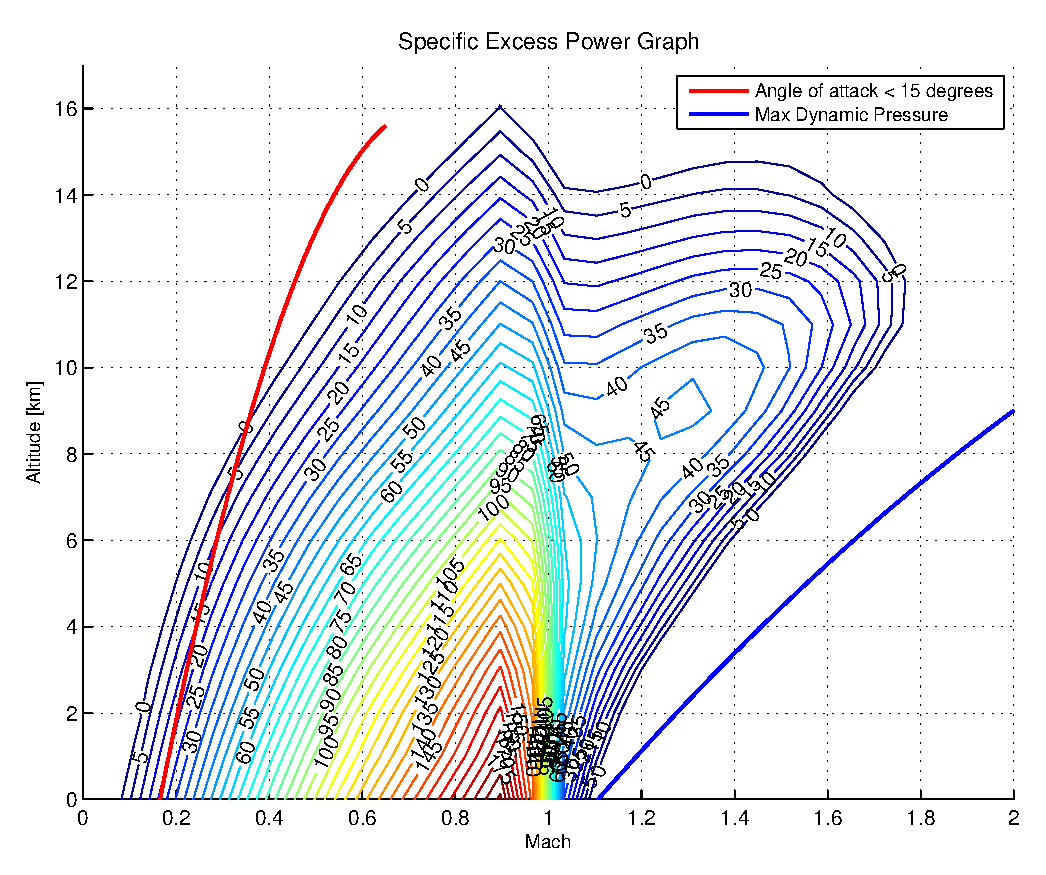
\includegraphics[width=1.2\textwidth]{SEP_Graph}
    \caption{SEP Graph}
    \label{fig:SEP_Graph}
\end{figure}

Graph \ref{fig:SEP_Graph} shows the contours of same Excess Power with regards to
the altitude of the airplane as well as the Mach number thus the velocity of the airplane.

Using the graph we can also determine the envelope limits corresponding to the maximum angle of attack
$(15^{\degree})$ and the maximum dynamic pressure corresponding to $1350 \sfrac{km}{h}$ at sea level which 
is $8.6133e+04 Pa$.

\subsection{Maximum altitude - Maximum Mach Number}
The maximum altitude and the maximum Mach Number at which the aircraft can fly level 
can be determined using \ref{fig:SEP_Graph}:

\begin{itemize*}
    \item Max. Altitude: 16 km
    \item Max Mach: 1.76
\end{itemize*}


%%%%%%%%%%%%%%%%%%%%%%%%%%%%%%%%%%%%%%%
%      MINIMUM TIME TO CLIMB          %
%%%%%%%%%%%%%%%%%%%%%%%%%%%%%%%%%%%%%%%
\section{Minimum time to climb}

\subsection{Computing $\gamma(t)$  - minimum time to climb}

\subsection{Trajectory for maximum Mach number in minimum time}

\subsection{Trajectory for maximum altitude in minimum time}





%%%%%%%%%%%%%%%%%%%%%%%%%%%%%%%%%%%%%%%
%             PART II                 %
%%%%%%%%%%%%%%%%%%%%%%%%%%%%%%%%%%%%%%%
\section{Derivation of $C_{l}$ rolling moment coefficient}
In this part of the project the rolling moment coefficient of the J35 Draken is to be calculated.
For the simulation, the model of fig.\ref{fig:model} was used:

\begin{figure}[H]
    \begin{center}
        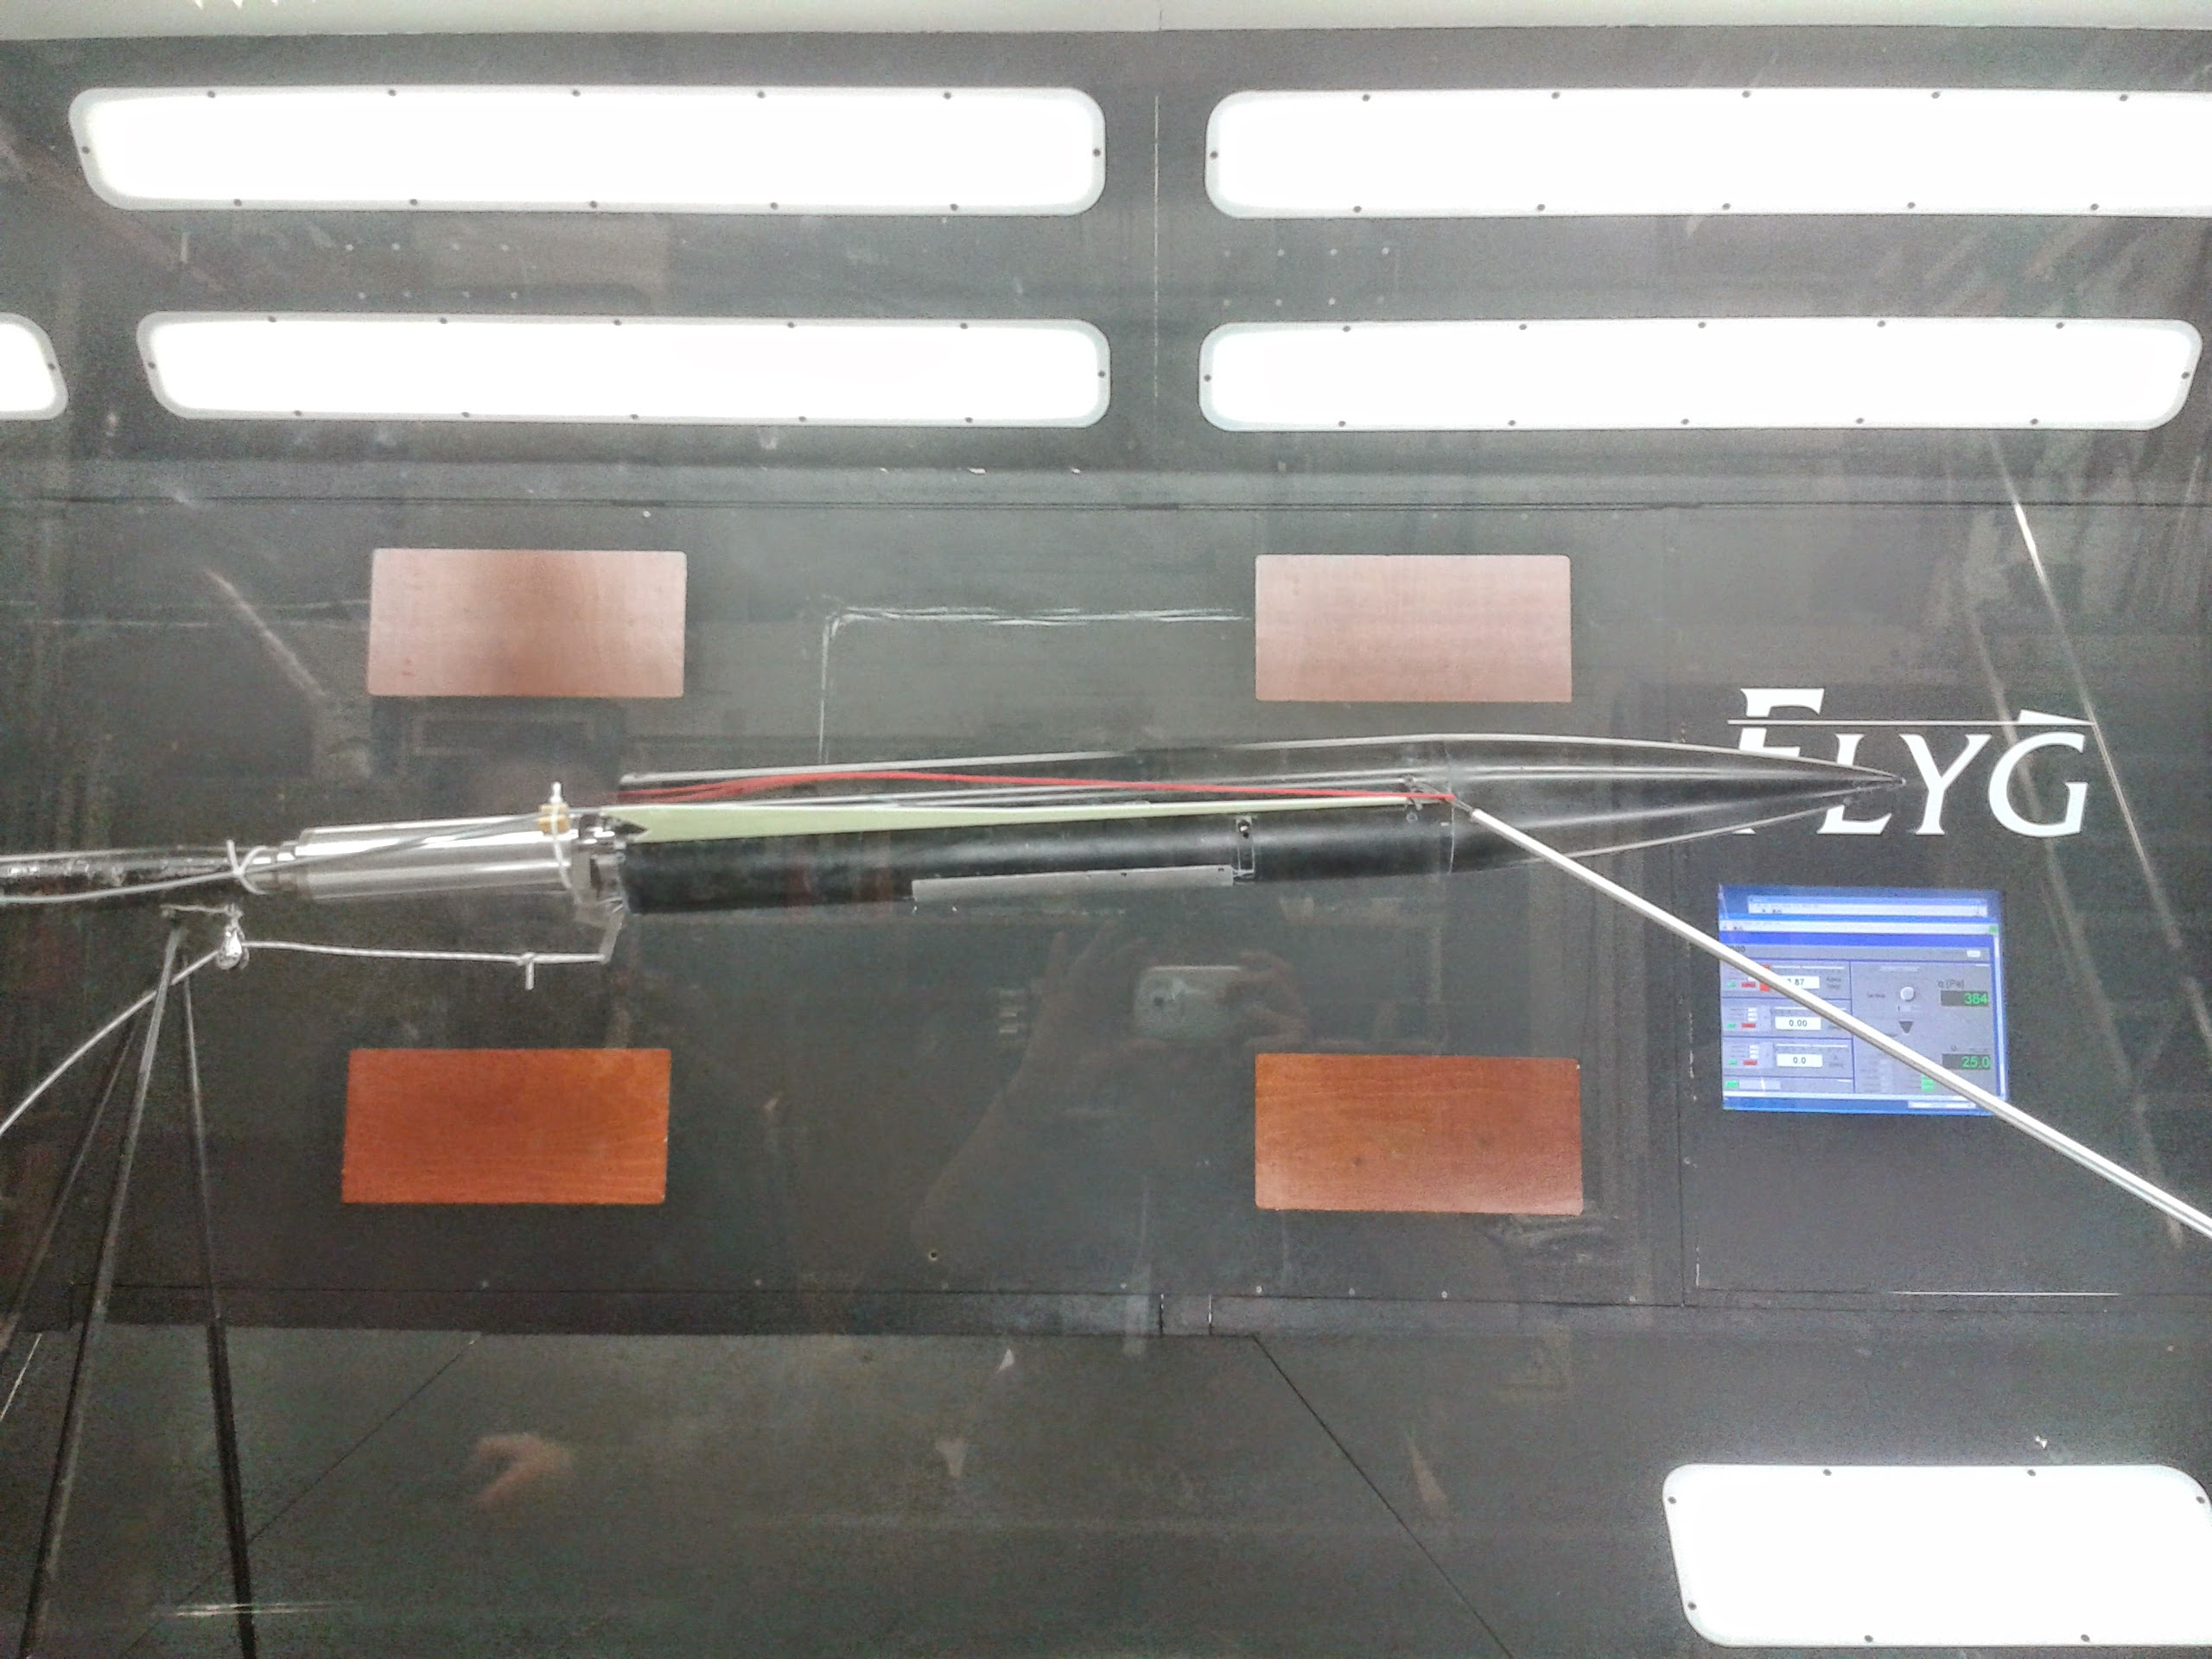
\includegraphics[width = 0.6\textwidth]{model.jpg} % Just THIS!!!
    \end{center}
    \caption{Picture of model during wind tunnel test}
    \label{fig:model}
\end{figure}

\subsection{Simulation Considerations}

The following can be stated when comparing the J35 Draken aircraft with the wind tunnel model used(fig.~\ref{fig:model})
\begin{itemize*}
    \item Apparently the major difference is the \textit{absence of the fin}. 
        This fact eventually caused considerable divergence between the values computed during the 
        simulation and the data extracted from Draken data diagramms provided.
    \item The wind tunnel model scale was 1:14.7 except for the bodywidth
        and noselength. 
\end{itemize*}


\subsection{Mathematical Modelling}
To proceed with the analysis and the computation of $C_{lp}, C_{l\beta}$ parameters, 
a valid mathematical model needs to be derived first. 
If We implement the Newton's second law for the rolling movement
we can derive equation \ref{eqn:newton_angular}.

\begin{equation}
    \Sigma T = I_{xx}\ddot{\phi} \Rightarrow 
    l - C\dot{\phi} - k\phi = I_{xx}\ddot{\phi},
    \label{eqn:newton_angular}
\end{equation}

\nomenclature{$I_{xx}$}{Rolling moment of inertia}%
\nomenclature{$C$}{Damping coefficient of aircraft rolling motion}%
\nomenclature{$q$}{Dynamical Pressure}%
\nomenclature{$C$}{Damping coefficient of aircraft rolling motion}%
\nomenclature{$k$}{Spring coefficient of aircraft rolling motion}%
\nomenclature{$p$}{Roll angle derivative}%
\nomenclature{$\rho$}{Density of air}%
\nomenclature{$u$}{Projection of velocity on the x-axis of airplane (Body-fixed system)}%
\nomenclature{$v$}{Projection of velocity on the y-axis of airplane (Body-fixed system)}%
\nomenclature{$w$}{Projection of velocity on the w-axis of airplane (Body-fixed system)}%

\noindent where $C\dot{\phi}$ is the moment exerted due to the (mechanical) damping and $k\phi$ is
the moment due to the (mechanical) spring stiffness of the device holding the airplane during the simulation.
For the calculation of the rolling moment the following equations can be used:
\begin{eqnarray}
    l &=& C_l q b S \label{eqn:roll_moment} \label{eqn:l}\\
    C_l &=&  C_{lp}\frac{pb}{2u} + C_{l\beta}\beta \label{eqn:cl}\\
    p &=&\dot{\phi} \notag\\
    q &=&  \frac{1}{2}\rho v^2 \notag
\end{eqnarray}

\nomenclature{$l$}{Rolling moment}%
\nomenclature{$C_l$}{Rolling moment coefficient}%

A sufficient model of calculating $C_l$ - the rolling moment coefficient - is given in equation
\ref{eqn:cl}. According to this, $C_l$ is a function of $C_{lp}$ the \textit{damping-in-roll}
coefficient and $C_{l\beta}$ the dihedral effect.
$C_{lp}$ expresses the resistance of the airplane to rolling 
\cite{etkin_dynamics_1972}, while $C_{l\beta}$ expresses the change in rolling moment 
coefficient per degree of change in the sideslip angle $\beta$. A sufficient relation to 
calculating $\beta$ can be the following:
\begin{equation}
    \beta = \alpha \phi
    \label{eqn:beta}
\end{equation}

\nomenclature{$\beta$}{Sideslip angle}%

\noindent If we now substitute the expression of rolling moment \ref{eqn:l} into the initial equation
\ref{eqn:newton_angular}, and move all the $\phi, \dot{\phi}$ terms to the other side of the equation
we can end up with the following second order differential equation:

\begin{equation}
    I_{xx}\ddot{\phi} + \dot{\phi}\big(C_{mech} - \frac{C_{lp}Sb^2q}{2u}\big) + \big(k - C_{l\beta}aqbS\big)\phi = 0
    \label{eqn:ode_used}
\end{equation}

\noindent The analytical solution of \ref{eqn:ode_used} for the general case of complex roots
(which is what we expect due to the oscillatory behavior of the model movement) is the following:

\begin{eqnarray}
    \phi &=&  c_1e^{\alpha' x}cos(\beta' x) + c_2e^{\alpha' x} sin(\beta' x) \label{eqn:phianal}\\
    \alpha' &=&  -\frac{\beta}{2\alpha} \notag\\
    \beta' &=&  \frac{\sqrt{4ac - b^2}}{2a} \notag\\
\end{eqnarray}

where $\alpha, \beta, c$ are the coefficients of \ref{eqn:ode_used} respectively:
\begin{eqnarray}
    \alpha &=& I_{xx} \label{eqn:alpha}\\
    \beta &=&  C_{mech} - \frac{C_{lp}Sb^2q}{2u} \label{eqn:beta}\\
    c &=&  k - C_{l\beta}aqbS \label{eqn:c}
\end{eqnarray}

\nomenclature{b}{Airplane Span}%
\nomenclature{S}{Airplane Surface Area}%
\nomenclature{$C_{lp}$}{Damping in Roll Coefficient}%
\nomenclature{$C_{l\beta}$}{Dihedral Effect}%

\noindent To get the analytical solution of the roll rate $\dot{\phi}$ we take the derivative 
of \ref{eqn:phianal}:

\begin{eqnarray}
    \dot{\phi} &=&   \big(-C_1 \beta' sin(\beta' x) + C_2 \beta' cos(\beta' x) \big) e^{\alpha' x} =\notag\\
     &=&  \beta'\big(-C_1+C_2\big)e^{\alpha'}x\big(sin(\beta'x) + cos(\beta'x)\big) = \notag\\
     &\Rightarrow& \big\{A = \beta' \big(-C_1+C_2\big) \quad \big\} \Rightarrow \notag\\
     \dot{\phi} &=& Ae^{\alpha'x}\big(sin(\beta'x) + cos(\beta'x)\big) \label{eqn:panal} = \notag\\
     &\Rightarrow&  \big\{asin(\theta) + bcos(\theta) = Rsin\big(\theta \pm \alpha\big)\big\}\Rightarrow \notag\\
     \dot{\phi} &=& Ae^{\alpha'x}\big(sin(\beta'x + \Theta \big) \label{eqn:panal} \label{eqn:panal}
\end{eqnarray}

\subsection{Derivation of \textit{damping-in-roll} derivative $C_{lp}$}

To derive the $C_{lp}$ parameter, we first need to extract information out of 
the experimental data gathered. The oscillation of the rolling motion can be modelled as a 
decaying sinusoidal function of time. Therefore we can fit an exponential sinusoidal function 
of the form~\ref{eqn:panal} in the data and estimate each parameter 
by using the least squares method.

The data fit procedure uses the Fourier transform to extract the basic frequency as well as the least squares method.
Figures~\ref{fig:datafit1},\ref{fig:datafit2} show some examples of the data fits that demonstrate the efficiency of the 
approximation algorithm used.

\begin{figure}[H]
        \centering
        \begin{subfigure}[b]{0.48\textwidth}
                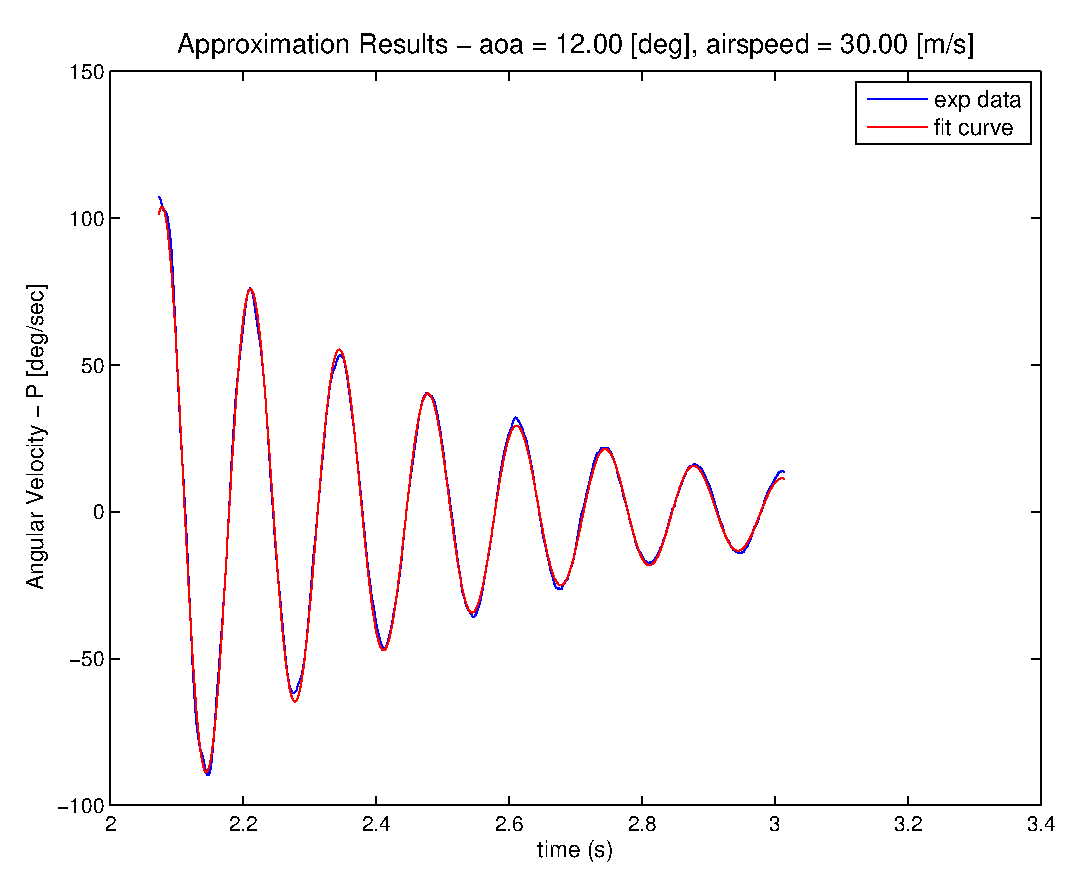
\includegraphics[width=\textwidth]{datafit_clp1}
                \caption{V = 35 $\sfrac{m}{s}$}
                \label{fig:datafit1}
        \end{subfigure}%
        ~
        \begin{subfigure}[b]{0.48\textwidth}
                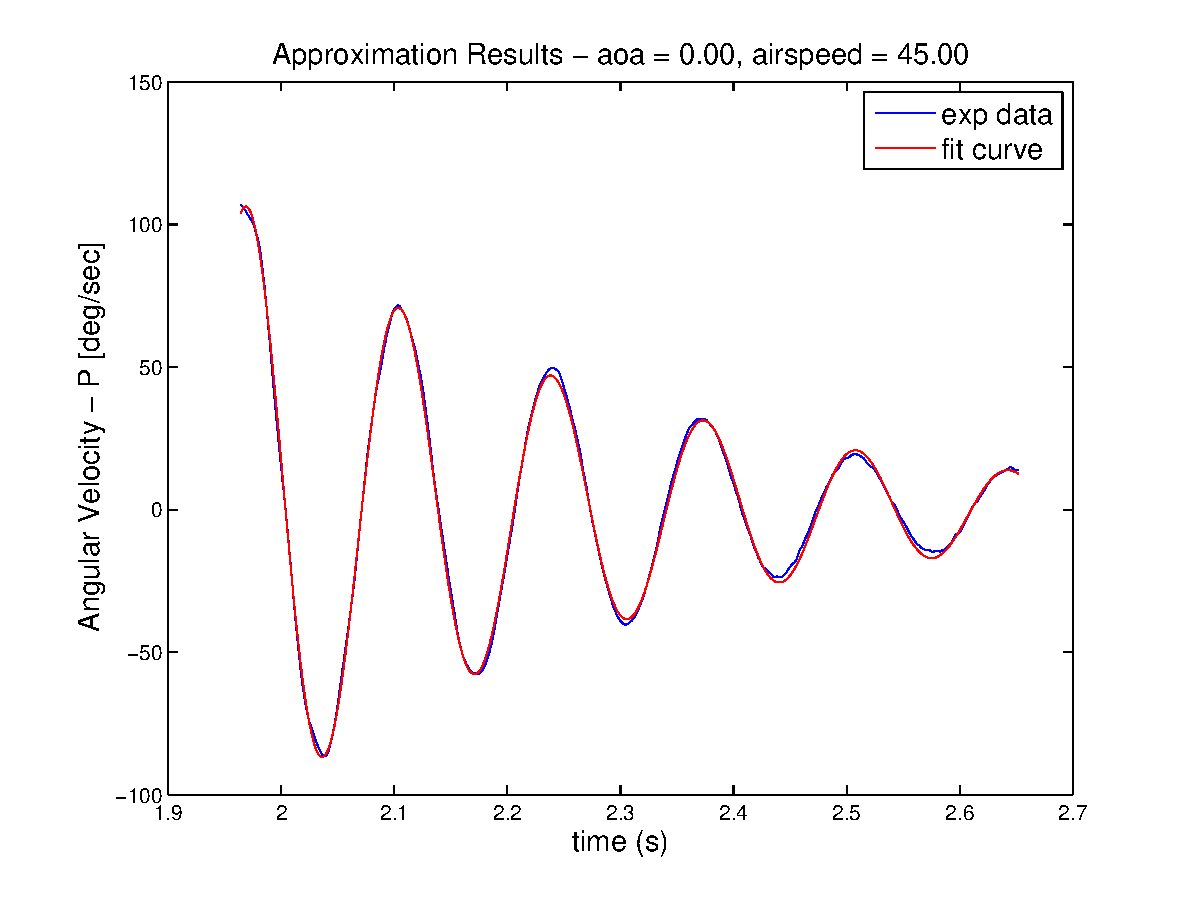
\includegraphics[width=\textwidth]{datafit_clp2}
                \caption{V = 45 $\sfrac{m}{s}$}
                \label{fig:datafit2}
        \end{subfigure}

        \caption{Examples of the data fitting procedure}
\end{figure}

To derive only the value of the $C_{lp}$ parameter we have to take into account \textit{only the data for $\alpha = 0$},
because otherwise $C_{l\beta}$ starts to play a role in the behavior of the oscilation (see eq.~\ref{eqn:ode_used}).

To extract the maximum amount of data and be as accurate as possible we \textit{process all the $\alpha = 0$ measurements taken during the laboratory sessions.}
\footnote{The reader is encouraged to refer to stiff.m of the code part for the actual implementation}.

The procedure can be summarised in the next steps:
\begin{enumerate}
    \item Calculation of $C_{mech}, I_{xx}$\footnote{I know that $I_{xx} = \sqrt{\frac{k}{\omega^2}}$ where k
    has already been determined experimentally.} using one of the  $\alpha = 0,\, V = 0$ measurements available.
    \item Approximation of the n-v \footnote{n is the damping coefficient, equivalent to $\beta'$ of eq.~\ref{eqn:panal}}curve by using a wide rage of velocities to calculate n-values and by using the least squares method.
    \item Calculation of the n-v  curve slope from which knowing every other quantity I can extract an estimation of the $C_{lp}$ value.
\end{enumerate}

Using this strategy we can now derive the approximation curve of the n-v points:
\begin{figure}[H]
    \begin{center}
        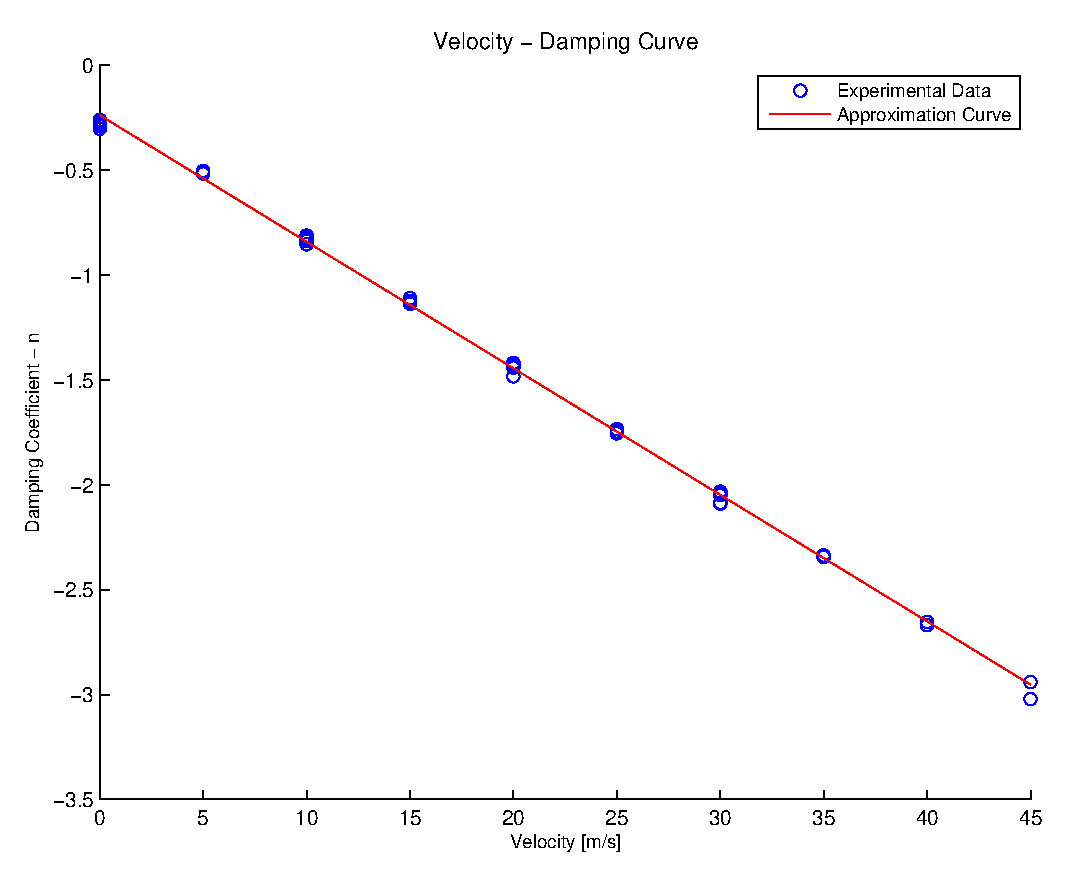
\includegraphics[width = \textwidth]{v_n_graph} % Just THIS!!!
    \end{center}
    \caption{Velocity - damping approximation curve}
    \label{fig:v_n_graph}
\end{figure}

\noindent From the above graph and using the methodology described in the previous steps we can now conclude to the value of $C_{lp}$:
\begin{equation}
    C_{lp} \simeq -0.190
\end{equation}

\noindent Since this value is (strictly) negative and is close to the data given for the real aircraft (for $\alpha = 0$), 
We can conclude that it is a logical estimation of the damping-in-roll coefficient.

\subsection{Derivation of the \textit{Dihedral effect} $C_{l\beta}$}

We use the same strategy as in the derivation of $C_{lp}$ to find a formula for 
calculating $C_{l\beta}$. $C_{l\beta}$ appers only in the formula of $\beta'$ (see eq. ~\ref{eqn:phianal})
which corresponds to the natural frequency of the aircraft oscillation. Executing the 
necessary computations, we can find an expression for the calculation of $C_{l\beta}$.

\begin{align}
    \omega_n &= \beta' = \frac{\sqrt{4\alpha c - \beta^2}}{2\alpha} \Rightarrow \notag\\
    \omega_n^2 &= \frac{4\alpha c - \beta^2}{4\alpha^2} \Rightarrow \notag\\
    &\Rightarrow \{\textrm{Substituting quantities from eq.~\ref{eqn:alpha}-\ref{eqn:c}} \}\Rightarrow \notag\\
    \omega_n^2 &= -\bigg(\frac{C_{l\beta}\alpha \rho bS}{2I_{xx}} + \frac{C_{lp}^2\rho S^2 b^4 \rho^2}{64I_{xx}^2}\bigg)V^2
    + \bigg(\frac{C_{mech}C_{lp}Sb^2\rho}{8I_{xx}^2}\bigg)V
    + \big(4I_{xx}k - C_{mech}^2\big) \label{eqn:wn2_V}
\end{align}

If we now fit the experimental data (V, $\omega_n^2$) into a quadratic polynomial model of the form 
$ax^2 + bx + c$ using the least squares method and extract the 
coefficients a, b, c we can find an analytical formula for $C_{l\beta}$.
So taking this into account and knowing that $C_{l\beta}$ appears in the expression
of the first coefficient of the $V-\omega_n^2$ curve, we end up with the following expresion:

\begin{equation}
    C_{l\beta} = -\bigg(\frac{2I_{xx}\times coeff(1)}{\alpha \rho bS} + 
    \frac{C_{lp}^2Sb^3I_{xx}}{32I_{xx}^2\alpha b}\bigg)
    \label{eqn:clb_calc}
\end{equation}

As we can see from eq~\ref{eqn:clb_calc} $C_{l\beta}$ is a function of the 
first coefficient of the fitting curve (coeff(1)), of $C_{lp}$ which was previously
calculated, and of $\alpha$. To proceed to the actual calculation, 
we fit quadratic polynomial curves over the $V-\omega^2$ pairs for each value of $\alpha$
and therefore caclulate the $C_{l\beta}$ values.
\footnote{We consider only the values of $\alpha$ for which sufficient experimental data has been gathered.
See stiff.m for the actual implementation}

Having executed the above procedure we end up with the following graphs 
for different $\alpha$ angles
\footnote{Some basic filtering was needed for the gathered experimental points. 
More specifically points that were outside the range of 3}

\begin{figure}[H]
    \begin{center}
        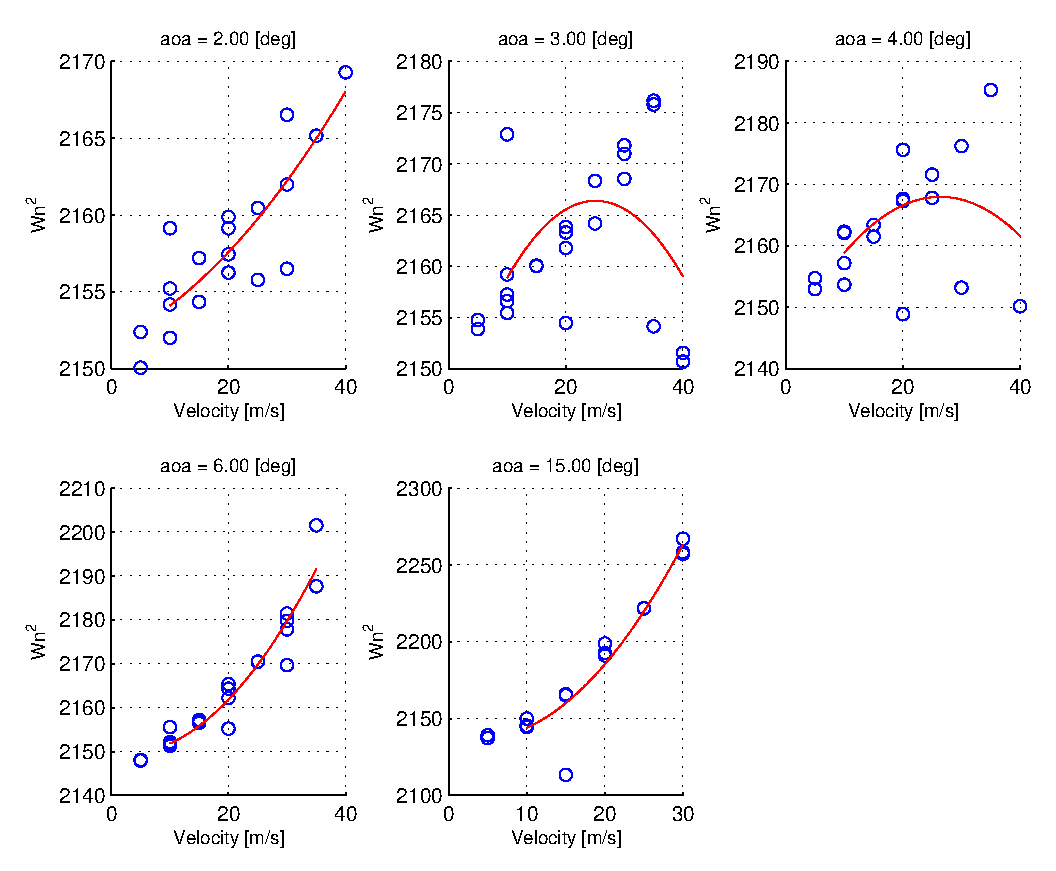
\includegraphics[width = \textwidth]{v_wmega2_graph} % Just THIS!!!
    \end{center}
    \caption{Fitting of polynomial curve into experimental data, for different $\alpha$ values}
    \label{fig:v_wmega2_graph}
\end{figure}

If we now extract $C_{l\beta}$ using eq.~\ref{eqn:clb_calc} we end up with the 
following values:

\begin{itemize}
    \item $\alpha = 2\degree\; \rightarrow \beta  = -0.0026$
    \item $\alpha = 3\degree\; \rightarrow \beta  = 0.0048$
    \item $\alpha = 4\degree\; \rightarrow \beta  = 0.0037$
    \item $\alpha = 6\degree\; \rightarrow \beta  = -0.0037$
    \item $\alpha = 15\degree\; \rightarrow \beta  = -0.0063$
\end{itemize}



%%%%%%%%%%%%%%%%%%%%%%%%%%%%%%%%%%%%%%%
%             PART III                %
%%%%%%%%%%%%%%%%%%%%%%%%%%%%%%%%%%%%%%%
\section{Stability and Control}

\nomenclature{$d_p$}{Thrust Level}%
\nomenclature{$d_e$}{Elevator setting}%
\nomenclature{$n_z$}{Load factor}%

\subsection{Equilibrium flight}
For the following analysis the following set of kinematic and dynamical
equations describes the motion of the aircraft sufficiently:
\begin{align}
    X - mgsin\theta &= m\big(\dot{u}^E + qw^E - rv^E \big)
    \label{full_longitudinal1}\\
    Y + mgcos\theta sin\phi &= m\bigl(\dot{v}^E+ ru^E - pw^E\bigr)\\
    Z + mgcos\theta cos\phi &= m\big(\dot{w}^E+ pv^E - qu^E\bigr)
    \label{full_longitudinal3}\\
    L &= I_x\dot{p} - I_{zx}\dot{r} + qr\bigl(I_z - I_y\bigr) - I_{zx}pq + qh_z' -
    rh_y'\\
    M &= I_y\dot{q} + rp\bigl(I_x - I_z\bigr)- I_{zx}\bigl(p^2-r^2\bigr) + rh_x' -
    ph_z'\\
    N &= I_z\dot{r} - I_{zx}\dot{p} + pq\bigl(I_y - I_x\bigr) + I_{zx}qr + ph_y'-qh_x'\\
    p &= \dot{\phi} - \dot{\psi}sin\theta\\
    q &= \dot{\theta}cos\phi + \dot{\psi}cos\theta sin\phi\\
    r &= \dot{\psi}cos\theta cos\phi- \dot{\theta} sin\phi \\
    \dot{\phi} &= p + \bigl(qsin\phi+ rcos\phi\bigr)tan\theta\\
    \dot{\theta} &= qcos\phi - rsin\phi\\
    \dot{\psi} &= \bigl(qsin\phi + rcos\phi\bigr)sec\theta\\
    \dot{x_E} &= u^Ecos\theta cos\psi + u^E\big(\sin\phi sin\theta cos\psi -
    cos\phi sin\psi\big) + \notag\\
     &+ w^E\big(\cos\phi sin\theta cos\psi - sin\phi sin\psi\big) \\
    \dot{y_E} &= v^Ecos\theta sin\psi + v^E\big(\sin\phi sin\theta sin\psi +
    cos\phi cos\psi\big) + \notag\\
     &+ w^E\big(\cos\phi sin\theta sin\psi - sin\phi cos\psi\big) \\
    \dot{z_E} &= -u^Esin\theta + v^Esin\phi cos\theta + w^Ecos\phi cos\theta
    \label{full_longitudinal15}\\
    u^E &= u + W_x\\
    v^E &= v + W_y\\
    w^E &= w + W_z \label{full_longitudinal18}
\end{align}

The above equations contain the following assumptions:
\begin{itemize}
\item The airplane is a rigid body, which may have attached to it any number of
rigid spinning rotors.
\item Cxz is a plane of mirror symmetry.
\item The axes of any spinning rotors are fixed in direction relative to the body
axes, and the rotors have constant angular speed relative to the body axes.
\end{itemize}

\subsubsection{Level Flight Trim Conditions}
As in the 1st part of the report, we have to first find a flyable situation for
the aircraft model. This is done by setting as many states of the above
equations to zero.
Equations~\ref{full_longitudinal1},\ref{full_longitudinal3},\ref{full_longitudinal15}
give 3 nonlinear algebraic equations. We also choose to set $\dot{M} = 0$ and
also know the formula for the velocity magnitude, $V = u^2 + v^2$ since $w = 0$.

So we end up with the following set of equations which we solve to compute the
trimmed state.

\begin{align}
    X - mgsin\theta &= 0\\
    Z + mgcos\theta &= 0\\
    -u^Esin\theta +  w^Ecos\theta &= 0\\
    \dot{M} &= 0\\
    V^2 &= u^2 + v^2
\end{align}
\begin{center}Set of nonlinear equations for trimmed state\end{center}

After finding an initial flyable situation, we linearise initial set of 
differential equations so that we end up with a system of the form:
\begin{align*}
    \underline{\dot{x}} &= \rttensor{J}\underline{\Delta x} +
    \rttensor{B}\underline{\Delta c}\\
    \underline{y} &= \rttensor{C}\underline{\Delta x}
\end{align*}
where for negligible input the differential equations are trimmed down to the 
$\underline{\dot{x}} = \rttensor{J}\,\underline{\Delta x}$ linear system.

Executing this procedure for mach numbers in the range of 0.1-0.7 and altitudes
0, 5000, 10000m we obtain the following graphs for $alpha, \delta_e,\delta_p$:

\begin{figure}[H]
    \centering
    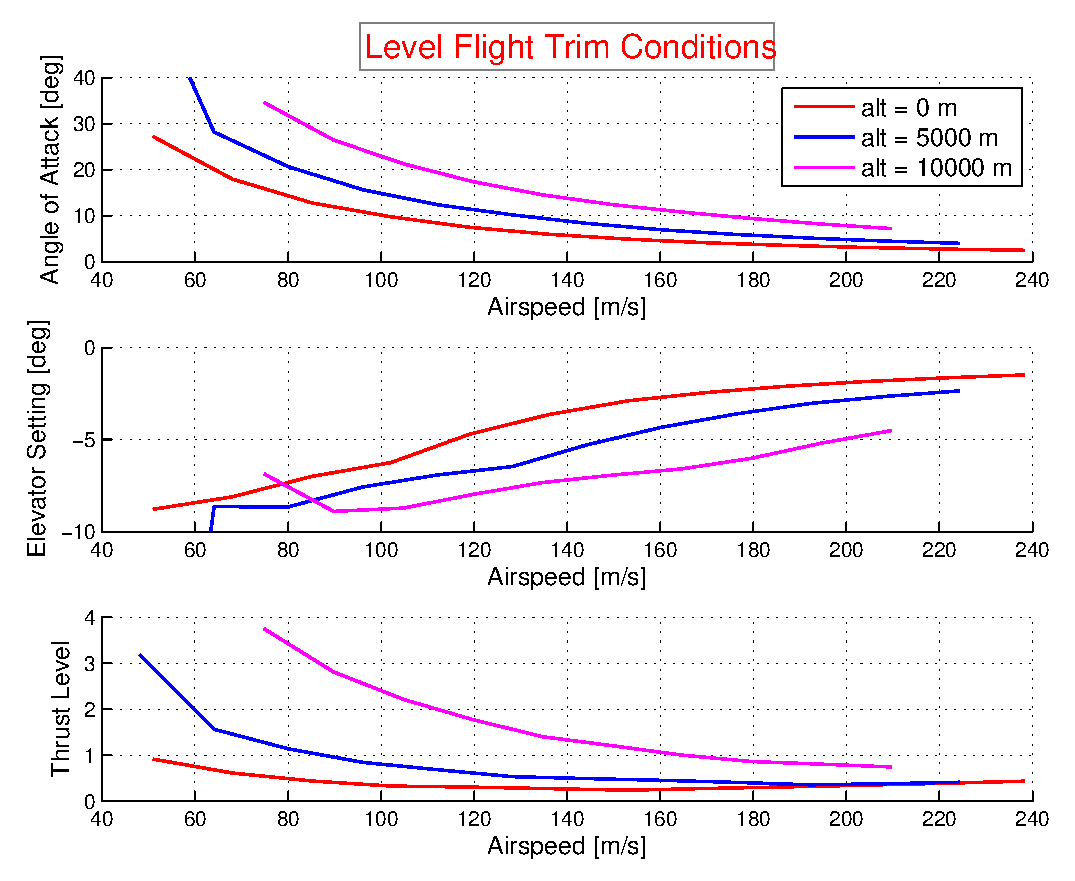
\includegraphics[width=1.0\textwidth]{equilibrium_conditions}
    \caption{$alpha, \delta_e,\delta_p$ for the trimmed Model}
\label{fig:equilibrium_conditions}
\end{figure}


\subsubsection{Center of gravity influence}
To investigate the influence of the center of gravity (xcg) on the elevator
angle we plot the equilibrium elevator as a function of the airspeed for
an altitude of 5000m  for two different xcg values (10.0, 10.3)m. 
The result is shown in fig~\ref{fig:xcg_investigation}.

\begin{figure}[H]
    \centering
    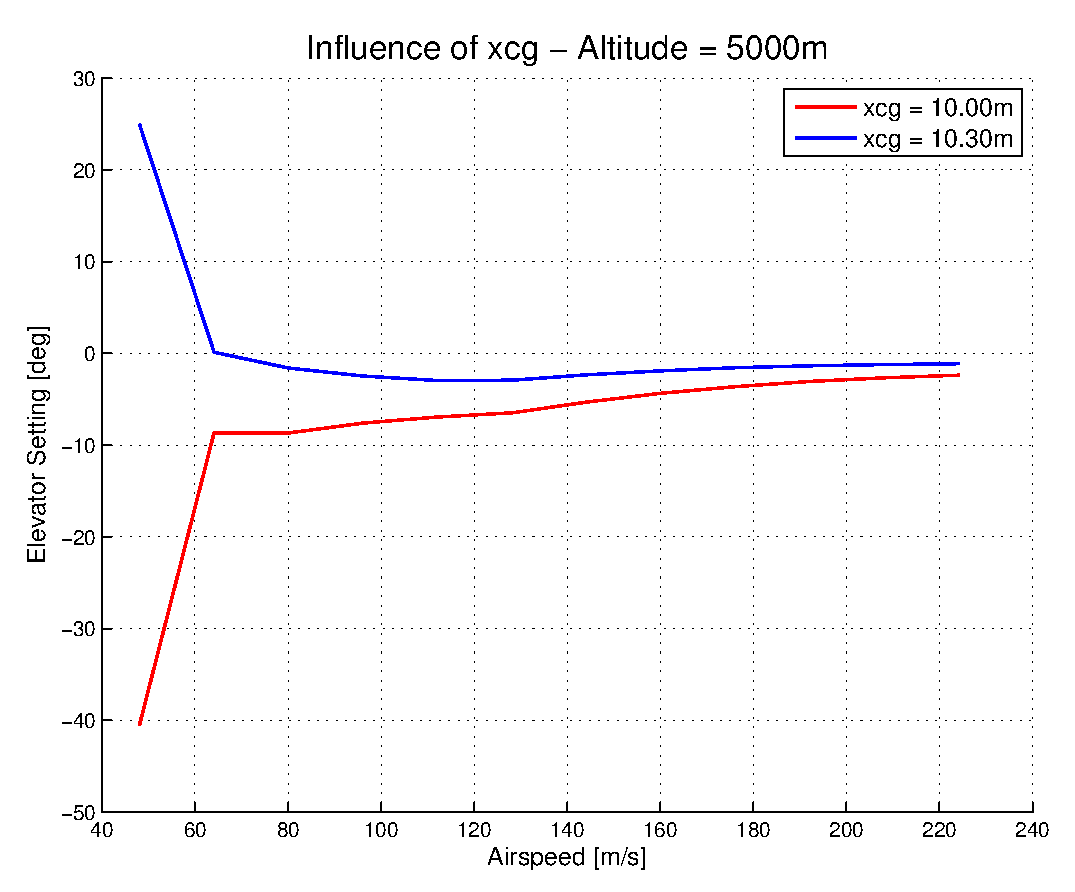
\includegraphics[width=1.0\textwidth]{xcg_investigation}
    \caption{Elevator setting for different cg positions}
    \label{fig:xcg_investigation}
\end{figure}

As we can see the sign of the setting changes to positive
\footnote{The elevator setting is defined as positive when the elevator goes
down.} at low airspeed. This is because the center of gravity has moved further
away from the tip of the aircraft comparing to the aerodynamic center, so a
torque emerges pushing the nose of the aircraft upwards. So in order for the
pitch-motion to be stable the elevator has to be positive as it is when xcg =
10.3m. So we can conclude that since the elevator setting is positive for a wide
range of airspeeds, xcg = 10.3m is not allowed position for the
aircraft. 

\subsubsection{Elevator per g}
The \textit{Elevator per g} can be computed using the following formula:
\begin{equation}
    Elevator_per_g = \frac{\Delta \delta e}{n-1}
    \label{eqn:elevator_per_g}
\end{equation}

In order to find it, we hold the velocity constant and the the thrust level zero,
for certain altitude and we implement a step input to the elevator. We then take
measure the difference in the load factor and therefore compute the elevator per
g from eq.~\ref{eqn:elevator_per_g}. 
We end up with the followign results which show that the epg goes down as the altitude increases.
\footnote{The results are also handed in as logfiles, see elevetor\_per\_g.log}:
\begin{itemize}
    \item $Altitude = 0 m\rightarrow Epg = 16.660$
    \item $Altitude = 5000 m \rightarrow Epg = 5.892$
    \item $Altitude = 10000 m \rightarrow Epg = 1.792$
\end{itemize}


\subsection{Linear stability analysis}

In order to investigate the linear stability of the aircraft we have to perform
an eigenvalue analysis for the Jacobian matrix computed during the trim problem
% todo add ref to previous equation

We compute the eigenvalues for altitudes 0, 5000, 10000m and for mach numbers
in the range of 0.1 - 0.7. We then plot the root locus graphs of the
eigenvalues with airspeed as a parameter.

\begin{figure}[H]
    \centering
    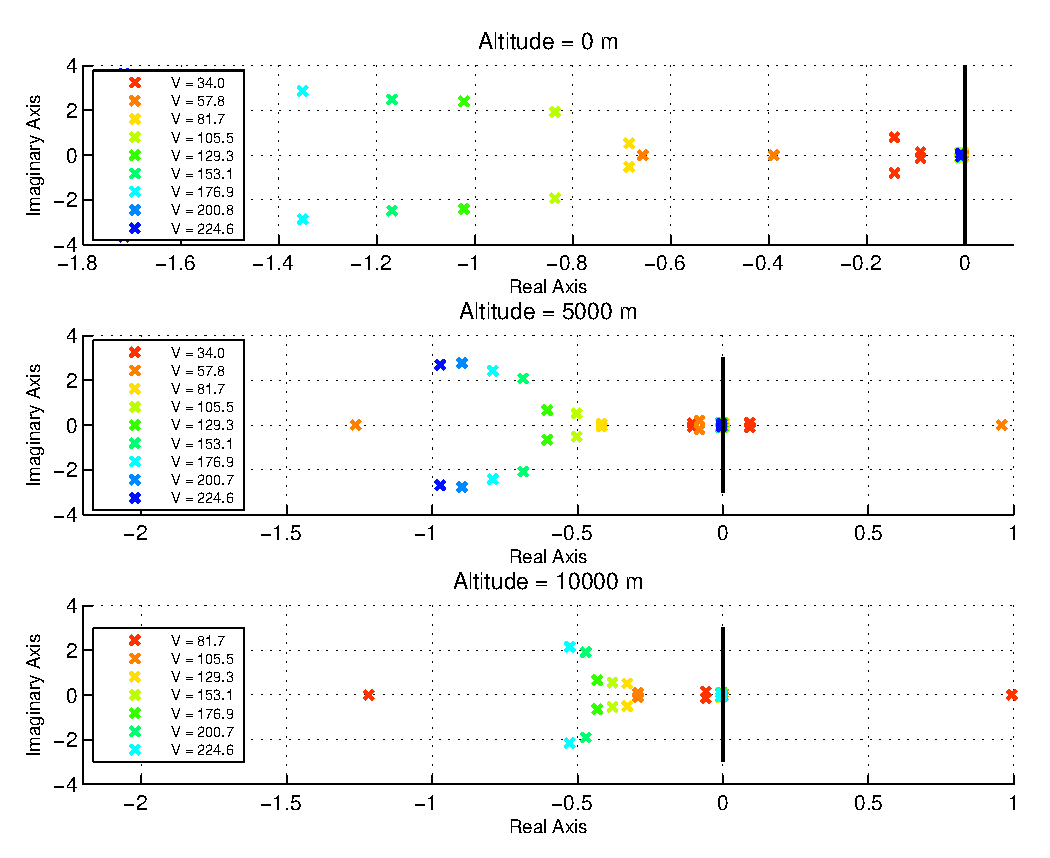
\includegraphics[width=1.0\textwidth]{linear_stability}
    \caption{Root Locus graph with regards to the airspeed}
    \label{fig:rlocus_airspeed}
\end{figure}

From fig.~\ref{fig:rlocus_airspeed} we can see that the linearised model
\textit{is not stable} for low airspeeds at alitude increases. More
specifically, at h = 5000m, the system is unstable for $V = 34\sfrac{m}{s}$
and $V = 57.8\sfrac{m}{s}$ and it becomes stable as the airspeed increases to 
$81.7\sfrac{m}{s}$. For h = 10000m on the other hand, we could not even reach an 
equilibrium trim state for $V \leq 81.7 {m}{s}$.

In particular, because we are interested in the stability of the longitudinal
movement we investigate the behavior of a submatrix of J that corresponds to the
longitudinal equations \cite{etkin_dynamics_1972}.

\begin{equation}
    J' = J\big(\Delta \dot{u}, \dot{w}, \dot{q}, \Delta
    \dot{theta}\big)\label{eqn:Jlong}
\end{equation}

For the stability analysis we compute the following based on J':
\begin{itemize*}
    \item Eigenvalues $\lambda$
    \item Eigenvectors $v$
    \item Oscillation frequencies $f$
    \item Time to half/double
\end{itemize*}

To compute the eigenvalues and eigenvectors, we implement the following
methodology:
\begin{align*}
    J' v &= \lambda v \Rightarrow\\
    \big(J'-\lambda I\big)v &= 0 \Rightarrow\\
    \abs{J' - \lambda I} &= 0 \numberthis \label{eqn:eigs_calc}
\end{align*}

Using eq~\eqref{eqn:eigs_calc} we can calculate the eigenvalues of the matrix by
solving the polynomial equation. Then to compute the corresponding eigenvector
we substitue each $\lambda$ calculated in the inital equation:
\begin{equation}
    \big(J'-\lambda_i I\big)v_i = 0,\; for\,i=1,\dots N,
    \label{eqn:eigvs_calc}
\end{equation}
where N is the total number of eigenvalues 

We also know that since the eigenvalues computed are of the form $n \pm
i\omega$, the frequency of each oscillation mode can be computed directly from
the eigenvalues:
\begin{equation}
    f = \frac{\omega}{2 \pi}
\end{equation}

The time to double/half can also be obtained using the following formula 
\cite{etkin_dynamics_1972}.

\begin{equation}
    t_{double} = t_{half} = \frac{log_e2}{\abs{n}}
    \label{eqn:time2double}
\end{equation}

Finally having computed the eigenvalues and the corresponding eigenvectors, the
oscillation modes can be computed using the following expression:
\begin{equation}
    \mathbf{X} = \mathbf{X_0}e^{\lambda t}
\end{equation}

The results of the eigenvalue analysis are presented in the appendix of the report
and are also handed in as logfiles.

\subsection{Nonlinear simulation}
We now simulate the behavior of the aircraft when executing each one of the
following maneuvers
\begin{itemize*}
    \item Looping
    \item Cobra maneuver
\end{itemize*}

We first run the simulation for 300 seconds with fixed inputs for the elevator
and the thrust level.
\begin{figure}[H]
    \centering
    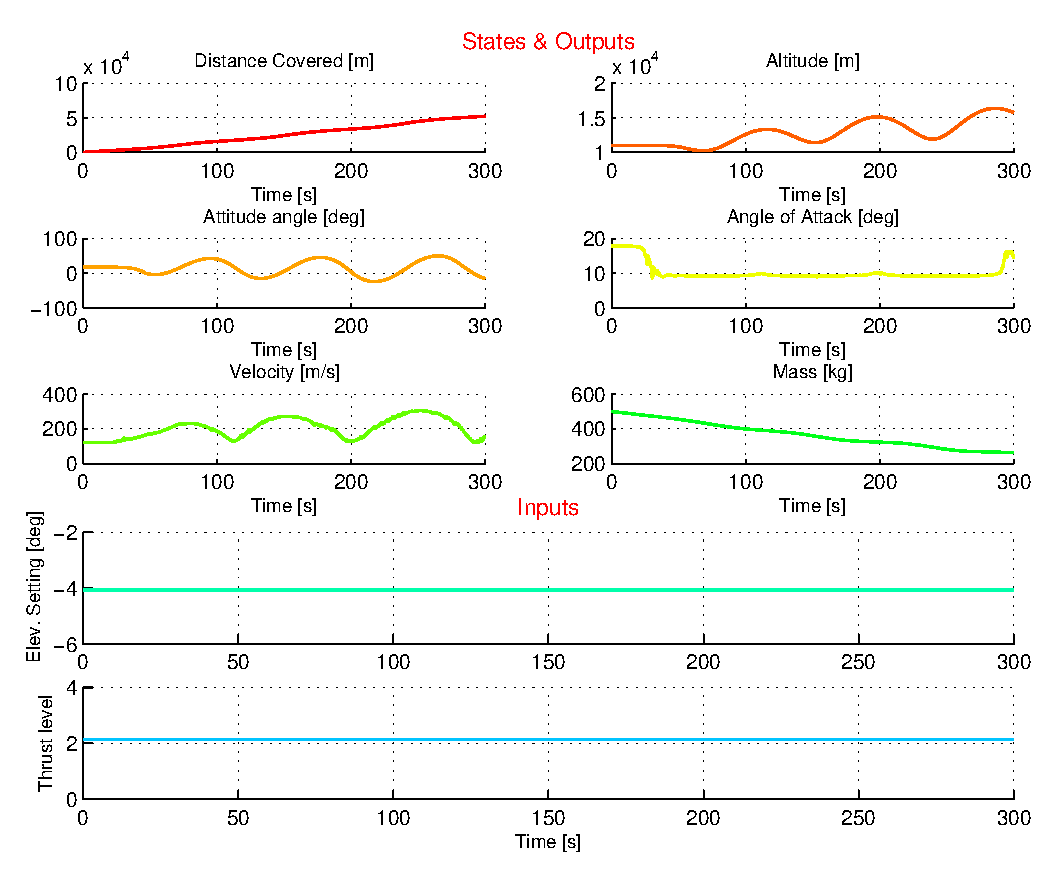
\includegraphics[width=1.0\textwidth]{nonlinear_sim}
    \caption{Simulation outcome for constant $\delta_e,\delta_p$}
    \label{fig:nonlinear_sim}
\end{figure}

As we can see, in the beginning (first 50s) aircrafts keeps a constant altitude
as wel as the other properties, but as the mass decreases, the aircraft starts
raising and velocity and attitude start oscilalting. The linear stability
analysis did not predict any divergence from the equilibrium point, because the
loss of mass was not included in the model.

An interesting point to make is that when the simulation is run with a
unacceptable cg position (e.g 10.3m) \textit{the altitude starts oscillating} with
increasing magnitude (see fig.\ref{fig:nonlinear2}) an indicator of unstable system behavior. If the xcg
increases even more, the time integration algorithm cannot find a valid solution
after a certain time.

\begin{figure}[H]
    \centering
    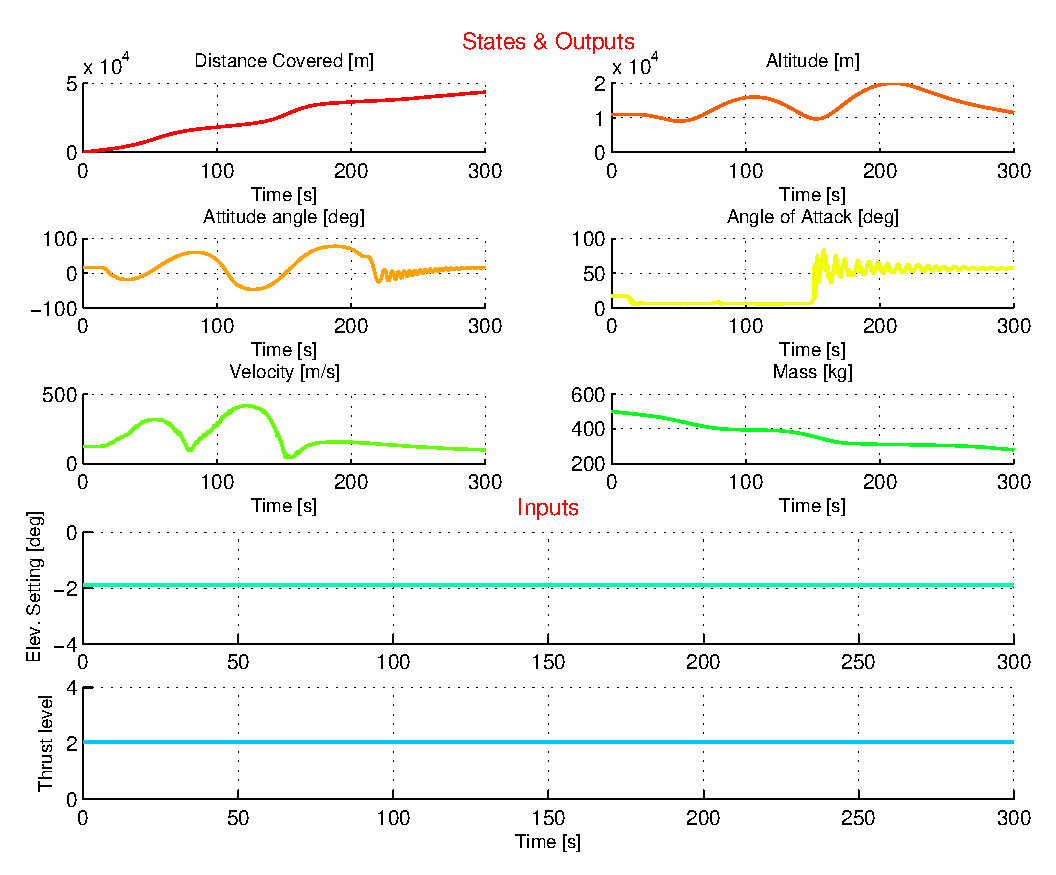
\includegraphics[width=1.0\textwidth]{nonlinear2}
    \caption{Nonlinear Simulation results for xcg = 10.3m}
    \label{fig:nonlinear2}
\end{figure}


\subsubsection{Looping}

The looping maneuver is perform by applying a negative elevator ($5-6\degree$) 
angle while having maximum thrust level. In this way the aircraft starts raising
in a curved trajectory until it reaches a maximum in an upside position. Then
maintaining the same elevator angle, after surpassing the max point of the
flight trajectory, we increase the thrust level so that when we reach the
initial altitude, we can maintain it in an equilibrium condition. 
\footnote{The elevator, thrust inputs are given in their respective csv files,
handed with the code}
The attempt of a loop maneuver is given 
in fig.~\ref{fig:looping}-\ref{fig:looping_status}


\begin{figure}[H]
    \centering
    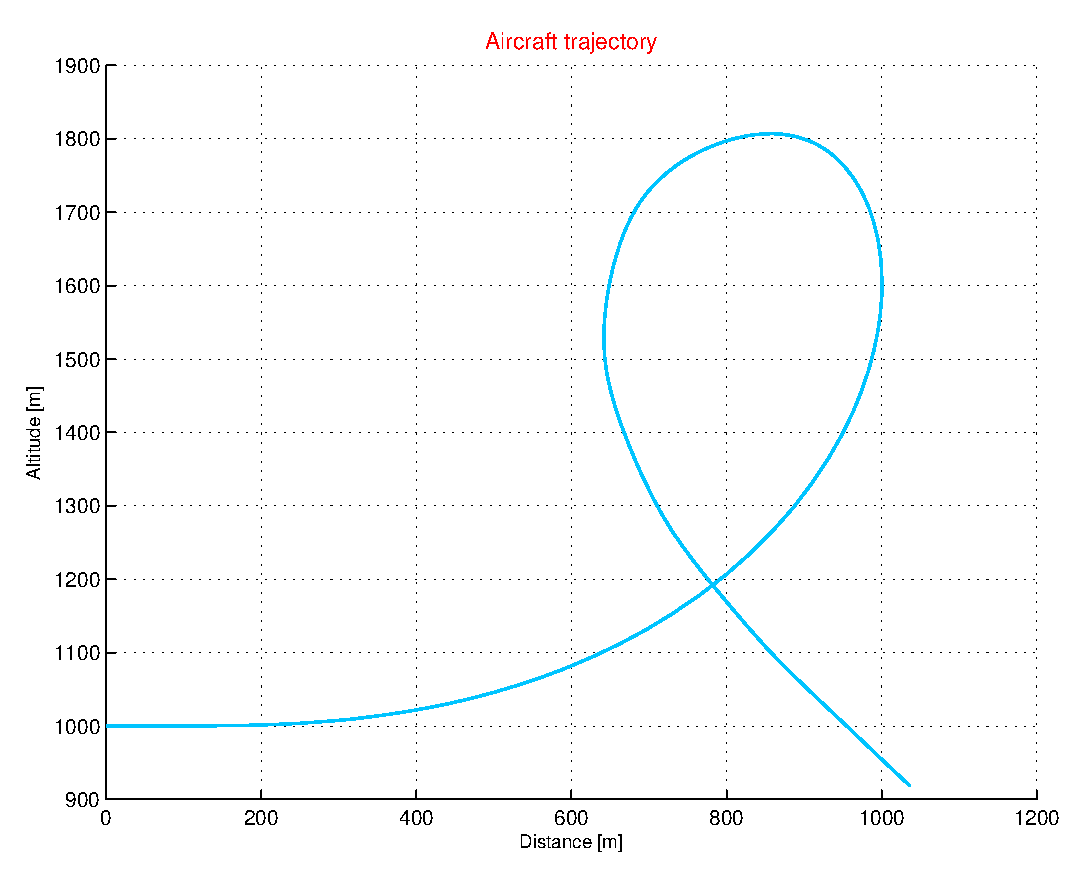
\includegraphics[width=\textwidth]{looping1}
        \caption{Looping Trajectory}
        \label{fig:looping}
\end{figure}
\begin{figure}[H]
    \centering
    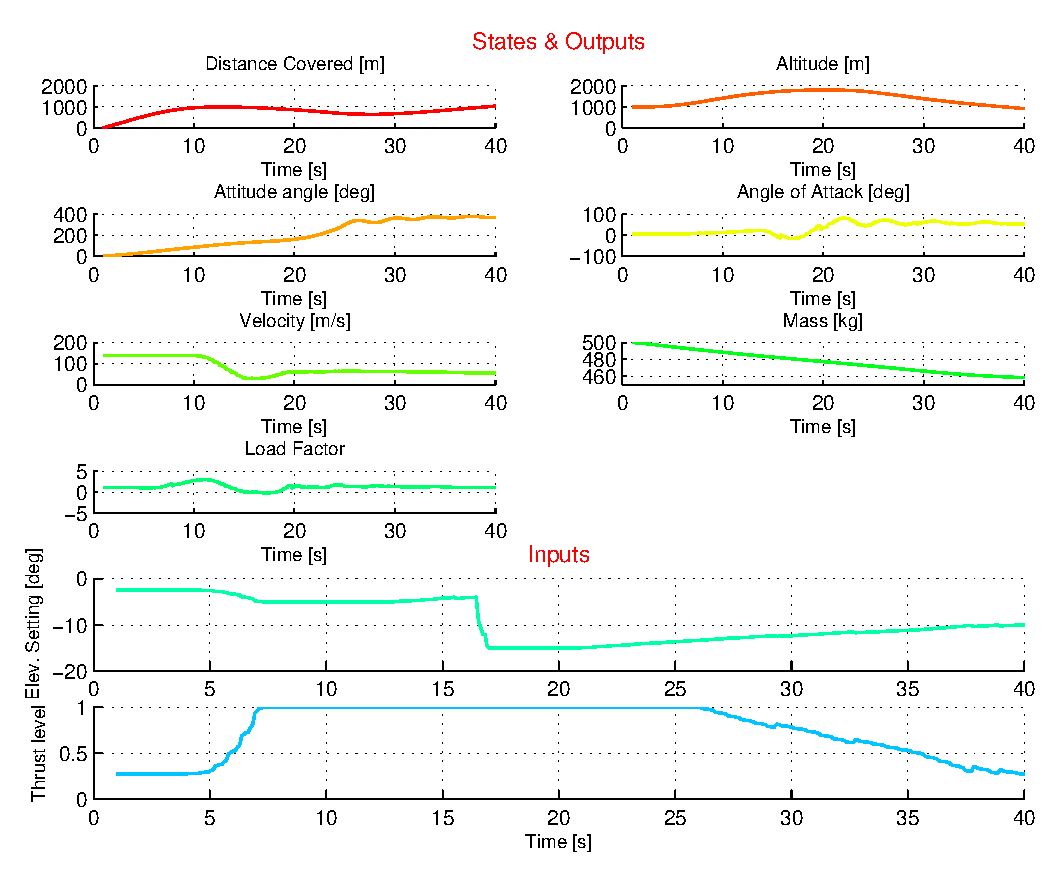
\includegraphics[width=\textwidth]{looping_status1}
    \caption{Parameters status during looping}
    \label{fig:looping_status}
\end{figure}

We can see that the roundness of the loop is sufficient, however we have
problems maintaining initial altitude after the loop.

\subsubsection{Cobra Maneuver}
In order to implement the cobra 





%----------------------------------------------------------------------------------------
%  BIBLIOGRAPHY
%----------------------------------------------------------------------------------------
\pagebreak
\nocite{*}
\bibliographystyle{plain}
\bibliography{j35_draken,riseofDraken,j35_database}

%%%%%%%%%%%%%%%%%%%%%%%%%%%%%%%%%%%%%%%
%             APPENDIX                %
%%%%%%%%%%%%%%%%%%%%%%%%%%%%%%%%%%%%%%%
\section{Appendix}
Below are the results of the eigenvalue analysis. For each altitude and the 
minimum and maximum mach  number each time the eigenvalues, the corresponding
eigenvectors, the oscillation frequencies and the double/half time are
presented.

\lstinputlisting[language={}]{../Project3/logfiles/eigenvalue_analysis.log}



\end{document}
